% Options for packages loaded elsewhere
\PassOptionsToPackage{unicode}{hyperref}
\PassOptionsToPackage{hyphens}{url}
%
\documentclass[
]{article}
\usepackage{amsmath,amssymb}
\usepackage{iftex}
\ifPDFTeX
  \usepackage[T1]{fontenc}
  \usepackage[utf8]{inputenc}
  \usepackage{textcomp} % provide euro and other symbols
\else % if luatex or xetex
  \usepackage{unicode-math} % this also loads fontspec
  \defaultfontfeatures{Scale=MatchLowercase}
  \defaultfontfeatures[\rmfamily]{Ligatures=TeX,Scale=1}
\fi
\usepackage{lmodern}
\ifPDFTeX\else
  % xetex/luatex font selection
\fi
% Use upquote if available, for straight quotes in verbatim environments
\IfFileExists{upquote.sty}{\usepackage{upquote}}{}
\IfFileExists{microtype.sty}{% use microtype if available
  \usepackage[]{microtype}
  \UseMicrotypeSet[protrusion]{basicmath} % disable protrusion for tt fonts
}{}
\makeatletter
\@ifundefined{KOMAClassName}{% if non-KOMA class
  \IfFileExists{parskip.sty}{%
    \usepackage{parskip}
  }{% else
    \setlength{\parindent}{0pt}
    \setlength{\parskip}{6pt plus 2pt minus 1pt}}
}{% if KOMA class
  \KOMAoptions{parskip=half}}
\makeatother
\usepackage{xcolor}
\usepackage[margin=1in]{geometry}
\usepackage{color}
\usepackage{fancyvrb}
\newcommand{\VerbBar}{|}
\newcommand{\VERB}{\Verb[commandchars=\\\{\}]}
\DefineVerbatimEnvironment{Highlighting}{Verbatim}{commandchars=\\\{\}}
% Add ',fontsize=\small' for more characters per line
\usepackage{framed}
\definecolor{shadecolor}{RGB}{248,248,248}
\newenvironment{Shaded}{\begin{snugshade}}{\end{snugshade}}
\newcommand{\AlertTok}[1]{\textcolor[rgb]{0.94,0.16,0.16}{#1}}
\newcommand{\AnnotationTok}[1]{\textcolor[rgb]{0.56,0.35,0.01}{\textbf{\textit{#1}}}}
\newcommand{\AttributeTok}[1]{\textcolor[rgb]{0.13,0.29,0.53}{#1}}
\newcommand{\BaseNTok}[1]{\textcolor[rgb]{0.00,0.00,0.81}{#1}}
\newcommand{\BuiltInTok}[1]{#1}
\newcommand{\CharTok}[1]{\textcolor[rgb]{0.31,0.60,0.02}{#1}}
\newcommand{\CommentTok}[1]{\textcolor[rgb]{0.56,0.35,0.01}{\textit{#1}}}
\newcommand{\CommentVarTok}[1]{\textcolor[rgb]{0.56,0.35,0.01}{\textbf{\textit{#1}}}}
\newcommand{\ConstantTok}[1]{\textcolor[rgb]{0.56,0.35,0.01}{#1}}
\newcommand{\ControlFlowTok}[1]{\textcolor[rgb]{0.13,0.29,0.53}{\textbf{#1}}}
\newcommand{\DataTypeTok}[1]{\textcolor[rgb]{0.13,0.29,0.53}{#1}}
\newcommand{\DecValTok}[1]{\textcolor[rgb]{0.00,0.00,0.81}{#1}}
\newcommand{\DocumentationTok}[1]{\textcolor[rgb]{0.56,0.35,0.01}{\textbf{\textit{#1}}}}
\newcommand{\ErrorTok}[1]{\textcolor[rgb]{0.64,0.00,0.00}{\textbf{#1}}}
\newcommand{\ExtensionTok}[1]{#1}
\newcommand{\FloatTok}[1]{\textcolor[rgb]{0.00,0.00,0.81}{#1}}
\newcommand{\FunctionTok}[1]{\textcolor[rgb]{0.13,0.29,0.53}{\textbf{#1}}}
\newcommand{\ImportTok}[1]{#1}
\newcommand{\InformationTok}[1]{\textcolor[rgb]{0.56,0.35,0.01}{\textbf{\textit{#1}}}}
\newcommand{\KeywordTok}[1]{\textcolor[rgb]{0.13,0.29,0.53}{\textbf{#1}}}
\newcommand{\NormalTok}[1]{#1}
\newcommand{\OperatorTok}[1]{\textcolor[rgb]{0.81,0.36,0.00}{\textbf{#1}}}
\newcommand{\OtherTok}[1]{\textcolor[rgb]{0.56,0.35,0.01}{#1}}
\newcommand{\PreprocessorTok}[1]{\textcolor[rgb]{0.56,0.35,0.01}{\textit{#1}}}
\newcommand{\RegionMarkerTok}[1]{#1}
\newcommand{\SpecialCharTok}[1]{\textcolor[rgb]{0.81,0.36,0.00}{\textbf{#1}}}
\newcommand{\SpecialStringTok}[1]{\textcolor[rgb]{0.31,0.60,0.02}{#1}}
\newcommand{\StringTok}[1]{\textcolor[rgb]{0.31,0.60,0.02}{#1}}
\newcommand{\VariableTok}[1]{\textcolor[rgb]{0.00,0.00,0.00}{#1}}
\newcommand{\VerbatimStringTok}[1]{\textcolor[rgb]{0.31,0.60,0.02}{#1}}
\newcommand{\WarningTok}[1]{\textcolor[rgb]{0.56,0.35,0.01}{\textbf{\textit{#1}}}}
\usepackage{graphicx}
\makeatletter
\def\maxwidth{\ifdim\Gin@nat@width>\linewidth\linewidth\else\Gin@nat@width\fi}
\def\maxheight{\ifdim\Gin@nat@height>\textheight\textheight\else\Gin@nat@height\fi}
\makeatother
% Scale images if necessary, so that they will not overflow the page
% margins by default, and it is still possible to overwrite the defaults
% using explicit options in \includegraphics[width, height, ...]{}
\setkeys{Gin}{width=\maxwidth,height=\maxheight,keepaspectratio}
% Set default figure placement to htbp
\makeatletter
\def\fps@figure{htbp}
\makeatother
\setlength{\emergencystretch}{3em} % prevent overfull lines
\providecommand{\tightlist}{%
  \setlength{\itemsep}{0pt}\setlength{\parskip}{0pt}}
\setcounter{secnumdepth}{-\maxdimen} % remove section numbering
\ifLuaTeX
  \usepackage{selnolig}  % disable illegal ligatures
\fi
\usepackage{bookmark}
\IfFileExists{xurl.sty}{\usepackage{xurl}}{} % add URL line breaks if available
\urlstyle{same}
\hypersetup{
  pdftitle={TP Final Estimacion Bayesiana},
  hidelinks,
  pdfcreator={LaTeX via pandoc}}

\title{TP Final Estimacion Bayesiana}
\usepackage{etoolbox}
\makeatletter
\providecommand{\subtitle}[1]{% add subtitle to \maketitle
  \apptocmd{\@title}{\par {\large #1 \par}}{}{}
}
\makeatother
\subtitle{Matias Moran y Matias Gangui}
\author{}
\date{\vspace{-2.5em}}

\begin{document}
\maketitle

En este trabajo final vamos a utilizar tecnicas de estimacion bayesiana
vistas en la materia para poder obtener y analizar informacion sobre
como se comportan los precios de mercado de los jugadores de futbol a
nivel internacional.

El dataset que usamos consiste del precio historico de mercado de
\textbf{8572} jugadores de futbol que alguna vez jugaron algun partido
en las competiciones mas importantes del mundo (UCL, Serie A, La Liga,
Premier y Bundesliga).

El dataset esta basado en una
\href{https://www.kaggle.com/datasets/davidcariboo/player-scores}{recopilacion}
de datos de la pagina \textbf{transfermarkt} la cual contiene
informacion historica de ligas, equipos y jugadores de futbol de todo el
mundo.

\section{Setup}\label{setup}

Importamos las librerias

\begin{Shaded}
\begin{Highlighting}[]
\CommentTok{\# Cargamos los paquetes}
\FunctionTok{library}\NormalTok{(bayesrules)}
\FunctionTok{library}\NormalTok{(tidyverse)}
\end{Highlighting}
\end{Shaded}

\begin{verbatim}
## -- Attaching core tidyverse packages ------------------------ tidyverse 2.0.0 --
## v dplyr     1.1.4     v readr     2.1.5
## v forcats   1.0.0     v stringr   1.5.1
## v ggplot2   3.5.1     v tibble    3.2.1
## v lubridate 1.9.3     v tidyr     1.3.1
## v purrr     1.0.2     
## -- Conflicts ------------------------------------------ tidyverse_conflicts() --
## x dplyr::filter() masks stats::filter()
## x dplyr::lag()    masks stats::lag()
## i Use the conflicted package (<http://conflicted.r-lib.org/>) to force all conflicts to become errors
\end{verbatim}

\begin{Shaded}
\begin{Highlighting}[]
\FunctionTok{library}\NormalTok{(rstanarm)}
\end{Highlighting}
\end{Shaded}

\begin{verbatim}
## Loading required package: Rcpp
## This is rstanarm version 2.32.1
## - See https://mc-stan.org/rstanarm/articles/priors for changes to default priors!
## - Default priors may change, so it's safest to specify priors, even if equivalent to the defaults.
## - For execution on a local, multicore CPU with excess RAM we recommend calling
##   options(mc.cores = parallel::detectCores())
\end{verbatim}

\begin{Shaded}
\begin{Highlighting}[]
\FunctionTok{library}\NormalTok{(bayesplot)}
\end{Highlighting}
\end{Shaded}

\begin{verbatim}
## This is bayesplot version 1.11.1
## - Online documentation and vignettes at mc-stan.org/bayesplot
## - bayesplot theme set to bayesplot::theme_default()
##    * Does _not_ affect other ggplot2 plots
##    * See ?bayesplot_theme_set for details on theme setting
\end{verbatim}

\begin{Shaded}
\begin{Highlighting}[]
\FunctionTok{library}\NormalTok{(tidybayes)}
\FunctionTok{library}\NormalTok{(broom.mixed)}
\FunctionTok{library}\NormalTok{(RColorBrewer)}
\end{Highlighting}
\end{Shaded}

Cargamos el dataset y hacemos feature engineering y reescalamos

\begin{Shaded}
\begin{Highlighting}[]
\CommentTok{\# Cargamos el dataset}
\NormalTok{football }\OtherTok{=} \FunctionTok{read.csv}\NormalTok{(}\StringTok{"players\_age\_valuation.csv"}\NormalTok{, }\AttributeTok{header =} \ConstantTok{TRUE}\NormalTok{)}

\NormalTok{football}\SpecialCharTok{$}\NormalTok{player\_id }\OtherTok{\textless{}{-}} \FunctionTok{as.character}\NormalTok{(football}\SpecialCharTok{$}\NormalTok{player\_id)}

\NormalTok{football }\OtherTok{\textless{}{-}}\NormalTok{ football }\SpecialCharTok{\%\textgreater{}\%}
  \FunctionTok{mutate}\NormalTok{(}\AttributeTok{age\_2 =}\NormalTok{ age}\SpecialCharTok{\^{}}\DecValTok{2}\NormalTok{)}
\NormalTok{football }\OtherTok{\textless{}{-}}\NormalTok{ football }\SpecialCharTok{\%\textgreater{}\%} 
  \FunctionTok{mutate}\NormalTok{(}\AttributeTok{log\_market\_value\_in\_eur =} \FunctionTok{log}\NormalTok{(market\_value\_in\_eur))}


\FunctionTok{head}\NormalTok{(football)}
\end{Highlighting}
\end{Shaded}

\begin{verbatim}
##   player_id               name age market_value_in_eur age_2
## 1      6893      Gabriel Tamas  20              900000   400
## 2        10     Miroslav Klose  26             7000000   676
## 3        26 Roman Weidenfeller  24             1500000   576
## 4        65   Dimitar Berbatov  23             8000000   529
## 5        77              Lúcio  26            13000000   676
## 6        80         Tom Starke  23              400000   529
##   log_market_value_in_eur
## 1                13.71015
## 2                15.76142
## 3                14.22098
## 4                15.89495
## 5                16.38046
## 6                12.89922
\end{verbatim}

\section{Data Exploration}\label{data-exploration}

Primero que nada vamos a ver la data de los jugadores para poder
entender mejor el problema y poder armar el modelo

\subsection{Distribucion de market
value}\label{distribucion-de-market-value}

Con el dataset completo de los 8572 jugadores para cada jugador vamos a
tomar el maximo, promedio y mediana de todos sus log market values
historicos en su carrera y vamos a hacer un histograma para ver como se
distribuyen los precios de los mismos.

\begin{Shaded}
\begin{Highlighting}[]
\NormalTok{players\_stats }\OtherTok{\textless{}{-}}\NormalTok{ football }\SpecialCharTok{\%\textgreater{}\%}
  \FunctionTok{group\_by}\NormalTok{(player\_id) }\SpecialCharTok{\%\textgreater{}\%}
  \FunctionTok{summarize}\NormalTok{(}
    \AttributeTok{max\_value =} \FunctionTok{max}\NormalTok{(log\_market\_value\_in\_eur, }\AttributeTok{na.rm =} \ConstantTok{TRUE}\NormalTok{),}
    \AttributeTok{median\_value =} \FunctionTok{median}\NormalTok{(log\_market\_value\_in\_eur, }\AttributeTok{na.rm =} \ConstantTok{TRUE}\NormalTok{),}
    \AttributeTok{mean\_value =} \FunctionTok{mean}\NormalTok{(log\_market\_value\_in\_eur, }\AttributeTok{na.rm =} \ConstantTok{TRUE}\NormalTok{)}
\NormalTok{  ) }\SpecialCharTok{\%\textgreater{}\%}
  \FunctionTok{ungroup}\NormalTok{() }\SpecialCharTok{\%\textgreater{}\%}
  \FunctionTok{pivot\_longer}\NormalTok{(}\AttributeTok{cols =} \FunctionTok{c}\NormalTok{(max\_value, median\_value, mean\_value), }
               \AttributeTok{names\_to =} \StringTok{"measure"}\NormalTok{, }
               \AttributeTok{values\_to =} \StringTok{"log\_market\_value"}\NormalTok{)}

\FunctionTok{ggplot}\NormalTok{(}\AttributeTok{data =}\NormalTok{ players\_stats, }\FunctionTok{aes}\NormalTok{(}\AttributeTok{x =}\NormalTok{ log\_market\_value, }\AttributeTok{fill =}\NormalTok{ measure)) }\SpecialCharTok{+}
  \FunctionTok{geom\_histogram}\NormalTok{(}\AttributeTok{color =} \StringTok{"black"}\NormalTok{, }\AttributeTok{alpha =} \FloatTok{0.7}\NormalTok{, }\AttributeTok{position =} \StringTok{"dodge"}\NormalTok{) }\SpecialCharTok{+}
  \FunctionTok{facet\_wrap}\NormalTok{(}\SpecialCharTok{\textasciitilde{}}\NormalTok{ measure, }\AttributeTok{scales =} \StringTok{"free"}\NormalTok{, }\AttributeTok{ncol =} \DecValTok{1}\NormalTok{) }\SpecialCharTok{+}
  \FunctionTok{ggtitle}\NormalTok{(}\StringTok{"Distribución de Valor de Mercado por Jugador (Máximo, Mediana, Promedio) (N=8572)"}\NormalTok{) }\SpecialCharTok{+}
  \FunctionTok{labs}\NormalTok{(}\AttributeTok{x =} \StringTok{"Log Valor de Mercado (en EUR)"}\NormalTok{, }\AttributeTok{y =} \StringTok{"Frecuencia"}\NormalTok{) }\SpecialCharTok{+}
  \FunctionTok{theme\_minimal}\NormalTok{() }\SpecialCharTok{+}
  \FunctionTok{theme}\NormalTok{(}\AttributeTok{legend.position =} \StringTok{"none"}\NormalTok{)}
\end{Highlighting}
\end{Shaded}

\begin{verbatim}
## `stat_bin()` using `bins = 30`. Pick better value with `binwidth`.
\end{verbatim}

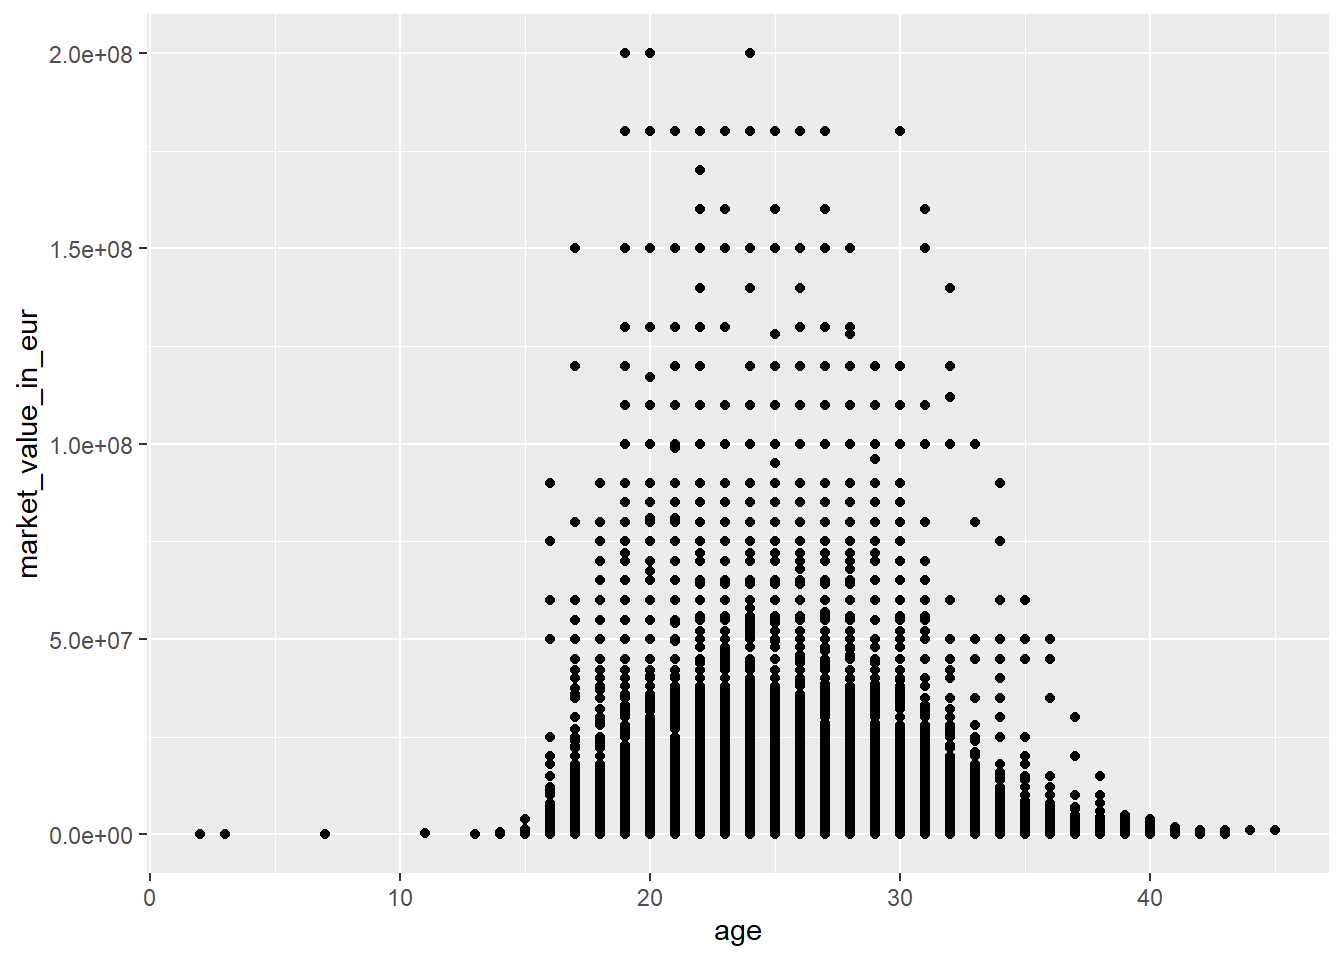
\includegraphics{output_files/figure-latex/unnamed-chunk-3-1.pdf}

Vemos que la forma del histograma de los precios (maximos, promedio y
mediana) de cada jugador tiene una forma normal, Esto nos dice que la
mayoria de los jugadores tienen precios parecidos y hay algunos pocos
que tienen precios muy altos y otros muy bajos.

Todo esto nos hace pensar que es razonable asignarle a cada jugador un
intercept normalmente distribuido a la hora de modelar.

Luego, vamos a ver como se comporta el precio de mercado de cada jugador
en el tiempo que dura su carrera, vamos a agarrar a 10 jugadores y a ver
su historial de precios.

\begin{Shaded}
\begin{Highlighting}[]
\FunctionTok{set.seed}\NormalTok{(}\DecValTok{314159}\NormalTok{)}

\NormalTok{players\_with\_history }\OtherTok{=}\NormalTok{ football }\SpecialCharTok{\%\textgreater{}\%}
  \FunctionTok{filter}\NormalTok{(age }\SpecialCharTok{\%in\%} \FunctionTok{c}\NormalTok{(}\DecValTok{20}\NormalTok{, }\DecValTok{35}\NormalTok{)) }\SpecialCharTok{\%\textgreater{}\%}
  \FunctionTok{group\_by}\NormalTok{(player\_id) }\SpecialCharTok{\%\textgreater{}\%}
  \FunctionTok{filter}\NormalTok{(}\FunctionTok{any}\NormalTok{(age }\SpecialCharTok{==} \DecValTok{20}\NormalTok{) }\SpecialCharTok{\&} \FunctionTok{any}\NormalTok{(age }\SpecialCharTok{==} \DecValTok{35}\NormalTok{)) }\SpecialCharTok{\%\textgreater{}\%}
  \FunctionTok{pull}\NormalTok{(player\_id) }\SpecialCharTok{\%\textgreater{}\%}
  \FunctionTok{unique}\NormalTok{()}

\CommentTok{\# El dataset cracks va a contener 54 jugadores de futbol de los 8572 originales, es el que vamos a usar para entrenar al modelo}
\NormalTok{cracks }\OtherTok{=}\NormalTok{ football[football}\SpecialCharTok{$}\NormalTok{player\_id }\SpecialCharTok{\%in\%} \FunctionTok{head}\NormalTok{(players\_with\_history, }\DecValTok{50}\NormalTok{),]}
\NormalTok{player\_ids }\OtherTok{=} \FunctionTok{c}\NormalTok{(}\DecValTok{28003}\NormalTok{, }\DecValTok{8198}\NormalTok{, }\DecValTok{68290}\NormalTok{, }\DecValTok{342229}\NormalTok{)}
\NormalTok{cracks }\OtherTok{=} \FunctionTok{rbind}\NormalTok{(cracks, football[football}\SpecialCharTok{$}\NormalTok{player\_id }\SpecialCharTok{\%in\%}\NormalTok{ player\_ids,])}

\CommentTok{\# Tomamos 10 jugadores del dataset y vemos sus historiales de precio}
\NormalTok{cracks\_10 }\OtherTok{=}\NormalTok{ football[football}\SpecialCharTok{$}\NormalTok{player\_id }\SpecialCharTok{\%in\%} \FunctionTok{head}\NormalTok{(players\_with\_history, }\DecValTok{10}\NormalTok{),]}

\FunctionTok{ggplot}\NormalTok{(}\AttributeTok{data =}\NormalTok{ cracks\_10, }\FunctionTok{aes}\NormalTok{(age, market\_value\_in\_eur, }\AttributeTok{color =}\NormalTok{ name)) }\SpecialCharTok{+}
  \FunctionTok{ggtitle}\NormalTok{(}\StringTok{"Precio de mercado historico por jugador (N = 10)"}\NormalTok{) }\SpecialCharTok{+}
  \FunctionTok{geom\_smooth}\NormalTok{(}\AttributeTok{method =} \StringTok{"loess"}\NormalTok{, }\AttributeTok{se =} \ConstantTok{FALSE}\NormalTok{) }\SpecialCharTok{+}
  \FunctionTok{theme}\NormalTok{(}\AttributeTok{legend.position =} \StringTok{"none"}\NormalTok{) }\SpecialCharTok{+}
  \FunctionTok{labs}\NormalTok{(}\AttributeTok{x=}\StringTok{"Edad"}\NormalTok{, }\AttributeTok{y=}\StringTok{"Valor (EUR)"}\NormalTok{) }\SpecialCharTok{+}
  \FunctionTok{scale\_y\_continuous}\NormalTok{(}\AttributeTok{labels =}\NormalTok{ scales}\SpecialCharTok{::}\FunctionTok{label\_dollar}\NormalTok{()) }\SpecialCharTok{+}
  \FunctionTok{lims}\NormalTok{(}\AttributeTok{y =} \FunctionTok{c}\NormalTok{(}\DecValTok{0}\NormalTok{,}\DecValTok{40000000}\NormalTok{))}
\end{Highlighting}
\end{Shaded}

\begin{verbatim}
## Scale for y is already present.
## Adding another scale for y, which will replace the existing scale.
## `geom_smooth()` using formula = 'y ~ x'
\end{verbatim}

\begin{verbatim}
## Warning: Removed 9 rows containing missing values or values outside the scale range
## (`geom_smooth()`).
\end{verbatim}

\includegraphics{output_files/figure-latex/unnamed-chunk-4-1.pdf}

\begin{Shaded}
\begin{Highlighting}[]
\FunctionTok{ggplot}\NormalTok{(}\AttributeTok{data =}\NormalTok{ cracks\_10, }\FunctionTok{aes}\NormalTok{(age, log\_market\_value\_in\_eur, }\AttributeTok{color =}\NormalTok{ name)) }\SpecialCharTok{+}
  \FunctionTok{ggtitle}\NormalTok{(}\StringTok{"Log{-}Precio de mercado historico por jugador (N = 10)"}\NormalTok{) }\SpecialCharTok{+}
  \FunctionTok{geom\_smooth}\NormalTok{(}\AttributeTok{method =} \StringTok{"loess"}\NormalTok{, }\AttributeTok{se =} \ConstantTok{FALSE}\NormalTok{) }\SpecialCharTok{+}
  \FunctionTok{theme}\NormalTok{(}\AttributeTok{legend.position =} \StringTok{"none"}\NormalTok{) }\SpecialCharTok{+}
  \FunctionTok{labs}\NormalTok{(}\AttributeTok{x=}\StringTok{"Edad"}\NormalTok{, }\AttributeTok{y=}\StringTok{"Log{-}Valor (EUR)"}\NormalTok{) }\SpecialCharTok{+}
  \FunctionTok{scale\_y\_continuous}\NormalTok{(}\AttributeTok{labels =}\NormalTok{ scales}\SpecialCharTok{::}\FunctionTok{label\_dollar}\NormalTok{()) }\SpecialCharTok{+}
  \FunctionTok{lims}\NormalTok{(}\AttributeTok{y =} \FunctionTok{c}\NormalTok{(}\DecValTok{10}\NormalTok{,}\DecValTok{18}\NormalTok{))}
\end{Highlighting}
\end{Shaded}

\begin{verbatim}
## Scale for y is already present.
## Adding another scale for y, which will replace the existing scale.
## `geom_smooth()` using formula = 'y ~ x'
\end{verbatim}

\includegraphics{output_files/figure-latex/unnamed-chunk-4-2.pdf}

\begin{Shaded}
\begin{Highlighting}[]
\FunctionTok{ggplot}\NormalTok{(cracks\_10, }\FunctionTok{aes}\NormalTok{(}\AttributeTok{x =}\NormalTok{ age, }\AttributeTok{y =}\NormalTok{ log\_market\_value\_in\_eur)) }\SpecialCharTok{+}
  \FunctionTok{geom\_point}\NormalTok{() }\SpecialCharTok{+}
  \FunctionTok{facet\_wrap}\NormalTok{(}\SpecialCharTok{\textasciitilde{}}\NormalTok{ player\_id) }\SpecialCharTok{+}
  \FunctionTok{ggtitle}\NormalTok{(}\StringTok{"Plot de 10 jugadores distintos"}\NormalTok{)}
\end{Highlighting}
\end{Shaded}

\includegraphics{output_files/figure-latex/unnamed-chunk-4-3.pdf} Vemos
como la tendencia general del historial de precios de un jugador tiene
una forma generalmente unimodal en la cual un jugador alcanza su maximo
precio de mercado y luego a medida que envejeze su precio va decayendo.

Esto nos hace pensar que una funcion cuadratica podria aproximar bien la
curva de precios de un jugador.

\section{Modelado}\label{modelado}

Dada la forma de los datos vamos a predecir el logaritmo del precio de
mercado de un jugador en base a su edad, vamos a hacer un modelo
jerarquico a nivel de jugador y vamos a tratar de modelar una relacion
cuadratica y vamos a asignar a cada jugador su propio intercept y
haremos que el intercept de cada jugador este normalmente distribuido
como vimos en el grafico anterior.

Este modelo tiene la limitacion de que va a hacer que todos los
jugadores tengan la misma tendencia a lo largo de su carrera y va a
capturar la relacion entre edad y precio para el jugador tipico.

\begin{Shaded}
\begin{Highlighting}[]
\FunctionTok{set.seed}\NormalTok{(}\DecValTok{314159}\NormalTok{)}

\NormalTok{quadratic\_fun }\OtherTok{\textless{}{-}} \ControlFlowTok{function}\NormalTok{(x, a, b, c) \{}
  \FunctionTok{return}\NormalTok{(a}\SpecialCharTok{*}\NormalTok{x}\SpecialCharTok{\^{}}\DecValTok{2} \SpecialCharTok{+}\NormalTok{ b}\SpecialCharTok{*}\NormalTok{x }\SpecialCharTok{+}\NormalTok{ c)}
\NormalTok{\}}

\FunctionTok{ggplot}\NormalTok{(}\AttributeTok{data =}\NormalTok{ cracks\_10, }\FunctionTok{aes}\NormalTok{(age, log\_market\_value\_in\_eur, }\AttributeTok{color =}\NormalTok{ name)) }\SpecialCharTok{+}
  \FunctionTok{ggtitle}\NormalTok{(}\StringTok{"Log{-}Precio de mercado historico por jugador (N = 10) con funcion cuadratica"}\NormalTok{) }\SpecialCharTok{+}
  \FunctionTok{geom\_smooth}\NormalTok{(}\AttributeTok{method =} \StringTok{"loess"}\NormalTok{, }\AttributeTok{se =} \ConstantTok{FALSE}\NormalTok{) }\SpecialCharTok{+}
  \FunctionTok{geom\_line}\NormalTok{(}\AttributeTok{data =} \FunctionTok{data.frame}\NormalTok{(}\AttributeTok{age =} \FunctionTok{seq}\NormalTok{(}\FunctionTok{min}\NormalTok{(cracks\_10}\SpecialCharTok{$}\NormalTok{age), }\FunctionTok{max}\NormalTok{(cracks\_10}\SpecialCharTok{$}\NormalTok{age), }\AttributeTok{length.out =} \DecValTok{100}\NormalTok{)), }
            \FunctionTok{aes}\NormalTok{(}\AttributeTok{x =}\NormalTok{ age, }\AttributeTok{y =} \FunctionTok{quadratic\_fun}\NormalTok{(age, }\SpecialCharTok{{-}}\FloatTok{0.05}\NormalTok{, }\FloatTok{2.7}\NormalTok{, }\SpecialCharTok{{-}}\DecValTok{19}\NormalTok{)), }\AttributeTok{color =} \StringTok{"black"}\NormalTok{, }\AttributeTok{size =} \FloatTok{1.5}\NormalTok{) }\SpecialCharTok{+}
  \FunctionTok{theme}\NormalTok{(}\AttributeTok{legend.position =} \StringTok{"none"}\NormalTok{) }\SpecialCharTok{+}
  \FunctionTok{labs}\NormalTok{(}\AttributeTok{x=}\StringTok{"Edad"}\NormalTok{, }\AttributeTok{y=}\StringTok{"Log{-}Valor (EUR)"}\NormalTok{) }\SpecialCharTok{+}
  \FunctionTok{scale\_y\_continuous}\NormalTok{(}\AttributeTok{labels =}\NormalTok{ scales}\SpecialCharTok{::}\FunctionTok{label\_dollar}\NormalTok{())}
\end{Highlighting}
\end{Shaded}

\begin{verbatim}
## Warning: Using `size` aesthetic for lines was deprecated in ggplot2 3.4.0.
## i Please use `linewidth` instead.
## This warning is displayed once every 8 hours.
## Call `lifecycle::last_lifecycle_warnings()` to see where this warning was
## generated.
\end{verbatim}

\begin{verbatim}
## `geom_smooth()` using formula = 'y ~ x'
\end{verbatim}

\includegraphics{output_files/figure-latex/unnamed-chunk-5-1.pdf}

La funcion cuadratica que vemos que puede llegar a aproximar bien a los
datos es \(y = -19 + 2.7x -0.05 x^2\) esta funcion sale de crear una que
este centrada aproximadamente en los picos de precio y tenga una
tendencia similar. Vamos a usar los coeficientes de esta funcion para
setear los priors de nuestro modelo

\subsection{Definicion del modelo:}\label{definicion-del-modelo}

\[
\text{data:} \quad Y_{{ij}}|\beta_{0j}, \beta_{1}, \beta_{2} ,\sigma_{y} \sim \mathcal{{N}}(\mu_{{ij}}, \sigma_{y}^{2}) \quad  \text{with} \quad  \mu_{{ij}} = \beta_{{0j}} + \beta_{{1}} \cdot X_{{ij}} + \beta_{{2}} \cdot X_{ij}^{2}
\]

\[
\text{priors:} \quad \beta_{0j}|\beta_{0},\sigma_{0} \sim \mathcal{{N}}(\beta_{0}, \sigma_{0}^{{2}})
\]

\[
\quad \quad \quad \quad \beta_{0c} \sim \mathcal{{N}}(-19, 20^2)
\]

\[
\quad \quad \quad \sigma_{0} \sim Exp(1)
\]

\[
\quad \quad \quad \quad \beta_{{1}} \sim \mathcal{{N}}(2.7, 5^{{2}})
\]

\[
\quad \quad \quad \quad \beta_{{2}} \sim \mathcal{{N}}(-0.05, 0.5^{{2}})
\]

\[
\quad \quad \quad \sigma_{y} \sim Exp(1)
\] Donde: \(Y_{ij}\) es el precio del jugador \(j\) a su edad \(i\)

\(X_{ij}\) es una edad del jugador \(j\)

\(\beta_{0j}\) es el intercept de la regresion para el jugador \(j\)

\(\beta_{1}\) el coeficiente global lineal (el cambio tipico lineal
entre edad y precio)

\(\beta_{2}\) el coeficiente global cuadratico (el cambio tipico
cuadratico entre edad y precio)

\(\sigma_{0}\) variabilidad entre los diferentes jugadores

\(\sigma_{y}\) variabilidad entre valores de un jugador y su modelo de
regresion, nos dice la fuerza de relacion entre edad y precio

\begin{Shaded}
\begin{Highlighting}[]
\FunctionTok{set.seed}\NormalTok{(}\DecValTok{314159}\NormalTok{)}

\NormalTok{model\_1 }\OtherTok{\textless{}{-}} \FunctionTok{stan\_glmer}\NormalTok{(}
\NormalTok{  log\_market\_value\_in\_eur }\SpecialCharTok{\textasciitilde{}}\NormalTok{ age }\SpecialCharTok{+}\NormalTok{ age\_2 }\SpecialCharTok{+}\NormalTok{ (}\DecValTok{1} \SpecialCharTok{|}\NormalTok{ player\_id),}
  \AttributeTok{data =}\NormalTok{ cracks,}
  \AttributeTok{family =}\NormalTok{ gaussian,}
  \AttributeTok{prior\_intercept =} \FunctionTok{normal}\NormalTok{(}\SpecialCharTok{{-}}\DecValTok{19}\NormalTok{, }\DecValTok{20}\NormalTok{, }\AttributeTok{autoscale =} \ConstantTok{TRUE}\NormalTok{), }\CommentTok{\#prior para los diferentes intercepts}
  \AttributeTok{prior =} \FunctionTok{normal}\NormalTok{(}\AttributeTok{location =} \FunctionTok{c}\NormalTok{(}\FloatTok{2.7}\NormalTok{, }\SpecialCharTok{{-}}\FloatTok{0.05}\NormalTok{), }\AttributeTok{scale =} \FunctionTok{c}\NormalTok{(}\DecValTok{5}\NormalTok{, }\FloatTok{0.5}\NormalTok{)), }\CommentTok{\#prior para los coeficientes}
  \AttributeTok{prior\_aux =} \FunctionTok{exponential}\NormalTok{(}\DecValTok{1}\NormalTok{, }\AttributeTok{autoscale =} \ConstantTok{TRUE}\NormalTok{), }\CommentTok{\#prior para sigma (ruido estadistico)}
  \AttributeTok{prior\_covariance =} \FunctionTok{decov}\NormalTok{(}\AttributeTok{reg =} \DecValTok{1}\NormalTok{, }\AttributeTok{conc =} \DecValTok{1}\NormalTok{, }\AttributeTok{shape =} \DecValTok{1}\NormalTok{, }\AttributeTok{scale =} \DecValTok{1}\NormalTok{), }\CommentTok{\# sigma\_0 equivalente a exp(1)}
  \AttributeTok{chains =} \DecValTok{4}\NormalTok{, }
  \AttributeTok{iter =} \DecValTok{10000}\NormalTok{, }
  \AttributeTok{seed =} \DecValTok{314159}
\NormalTok{)}
\end{Highlighting}
\end{Shaded}

\begin{verbatim}
## 
## SAMPLING FOR MODEL 'continuous' NOW (CHAIN 1).
## Chain 1: 
## Chain 1: Gradient evaluation took 0.0003 seconds
## Chain 1: 1000 transitions using 10 leapfrog steps per transition would take 3 seconds.
## Chain 1: Adjust your expectations accordingly!
## Chain 1: 
## Chain 1: 
## Chain 1: Iteration:    1 / 10000 [  0%]  (Warmup)
## Chain 1: Iteration: 1000 / 10000 [ 10%]  (Warmup)
## Chain 1: Iteration: 2000 / 10000 [ 20%]  (Warmup)
## Chain 1: Iteration: 3000 / 10000 [ 30%]  (Warmup)
## Chain 1: Iteration: 4000 / 10000 [ 40%]  (Warmup)
## Chain 1: Iteration: 5000 / 10000 [ 50%]  (Warmup)
## Chain 1: Iteration: 5001 / 10000 [ 50%]  (Sampling)
## Chain 1: Iteration: 6000 / 10000 [ 60%]  (Sampling)
## Chain 1: Iteration: 7000 / 10000 [ 70%]  (Sampling)
## Chain 1: Iteration: 8000 / 10000 [ 80%]  (Sampling)
## Chain 1: Iteration: 9000 / 10000 [ 90%]  (Sampling)
## Chain 1: Iteration: 10000 / 10000 [100%]  (Sampling)
## Chain 1: 
## Chain 1:  Elapsed Time: 64.776 seconds (Warm-up)
## Chain 1:                30.869 seconds (Sampling)
## Chain 1:                95.645 seconds (Total)
## Chain 1: 
## 
## SAMPLING FOR MODEL 'continuous' NOW (CHAIN 2).
## Chain 2: 
## Chain 2: Gradient evaluation took 9.9e-05 seconds
## Chain 2: 1000 transitions using 10 leapfrog steps per transition would take 0.99 seconds.
## Chain 2: Adjust your expectations accordingly!
## Chain 2: 
## Chain 2: 
## Chain 2: Iteration:    1 / 10000 [  0%]  (Warmup)
## Chain 2: Iteration: 1000 / 10000 [ 10%]  (Warmup)
## Chain 2: Iteration: 2000 / 10000 [ 20%]  (Warmup)
## Chain 2: Iteration: 3000 / 10000 [ 30%]  (Warmup)
## Chain 2: Iteration: 4000 / 10000 [ 40%]  (Warmup)
## Chain 2: Iteration: 5000 / 10000 [ 50%]  (Warmup)
## Chain 2: Iteration: 5001 / 10000 [ 50%]  (Sampling)
## Chain 2: Iteration: 6000 / 10000 [ 60%]  (Sampling)
## Chain 2: Iteration: 7000 / 10000 [ 70%]  (Sampling)
## Chain 2: Iteration: 8000 / 10000 [ 80%]  (Sampling)
## Chain 2: Iteration: 9000 / 10000 [ 90%]  (Sampling)
## Chain 2: Iteration: 10000 / 10000 [100%]  (Sampling)
## Chain 2: 
## Chain 2:  Elapsed Time: 72.657 seconds (Warm-up)
## Chain 2:                27.437 seconds (Sampling)
## Chain 2:                100.094 seconds (Total)
## Chain 2: 
## 
## SAMPLING FOR MODEL 'continuous' NOW (CHAIN 3).
## Chain 3: 
## Chain 3: Gradient evaluation took 9.6e-05 seconds
## Chain 3: 1000 transitions using 10 leapfrog steps per transition would take 0.96 seconds.
## Chain 3: Adjust your expectations accordingly!
## Chain 3: 
## Chain 3: 
## Chain 3: Iteration:    1 / 10000 [  0%]  (Warmup)
## Chain 3: Iteration: 1000 / 10000 [ 10%]  (Warmup)
## Chain 3: Iteration: 2000 / 10000 [ 20%]  (Warmup)
## Chain 3: Iteration: 3000 / 10000 [ 30%]  (Warmup)
## Chain 3: Iteration: 4000 / 10000 [ 40%]  (Warmup)
## Chain 3: Iteration: 5000 / 10000 [ 50%]  (Warmup)
## Chain 3: Iteration: 5001 / 10000 [ 50%]  (Sampling)
## Chain 3: Iteration: 6000 / 10000 [ 60%]  (Sampling)
## Chain 3: Iteration: 7000 / 10000 [ 70%]  (Sampling)
## Chain 3: Iteration: 8000 / 10000 [ 80%]  (Sampling)
## Chain 3: Iteration: 9000 / 10000 [ 90%]  (Sampling)
## Chain 3: Iteration: 10000 / 10000 [100%]  (Sampling)
## Chain 3: 
## Chain 3:  Elapsed Time: 61.527 seconds (Warm-up)
## Chain 3:                28.149 seconds (Sampling)
## Chain 3:                89.676 seconds (Total)
## Chain 3: 
## 
## SAMPLING FOR MODEL 'continuous' NOW (CHAIN 4).
## Chain 4: 
## Chain 4: Gradient evaluation took 9.4e-05 seconds
## Chain 4: 1000 transitions using 10 leapfrog steps per transition would take 0.94 seconds.
## Chain 4: Adjust your expectations accordingly!
## Chain 4: 
## Chain 4: 
## Chain 4: Iteration:    1 / 10000 [  0%]  (Warmup)
## Chain 4: Iteration: 1000 / 10000 [ 10%]  (Warmup)
## Chain 4: Iteration: 2000 / 10000 [ 20%]  (Warmup)
## Chain 4: Iteration: 3000 / 10000 [ 30%]  (Warmup)
## Chain 4: Iteration: 4000 / 10000 [ 40%]  (Warmup)
## Chain 4: Iteration: 5000 / 10000 [ 50%]  (Warmup)
## Chain 4: Iteration: 5001 / 10000 [ 50%]  (Sampling)
## Chain 4: Iteration: 6000 / 10000 [ 60%]  (Sampling)
## Chain 4: Iteration: 7000 / 10000 [ 70%]  (Sampling)
## Chain 4: Iteration: 8000 / 10000 [ 80%]  (Sampling)
## Chain 4: Iteration: 9000 / 10000 [ 90%]  (Sampling)
## Chain 4: Iteration: 10000 / 10000 [100%]  (Sampling)
## Chain 4: 
## Chain 4:  Elapsed Time: 61.594 seconds (Warm-up)
## Chain 4:                26.797 seconds (Sampling)
## Chain 4:                88.391 seconds (Total)
## Chain 4:
\end{verbatim}

Generamos posibles regresiones usando samples del prior para ver si el
modelo es coherente

\begin{Shaded}
\begin{Highlighting}[]
\NormalTok{model\_1\_prior }\OtherTok{\textless{}{-}} \FunctionTok{update}\NormalTok{(model\_1, }\AttributeTok{prior\_PD =} \ConstantTok{TRUE}\NormalTok{)}
\end{Highlighting}
\end{Shaded}

\begin{verbatim}
## 
## SAMPLING FOR MODEL 'continuous' NOW (CHAIN 1).
## Chain 1: 
## Chain 1: Gradient evaluation took 2e-05 seconds
## Chain 1: 1000 transitions using 10 leapfrog steps per transition would take 0.2 seconds.
## Chain 1: Adjust your expectations accordingly!
## Chain 1: 
## Chain 1: 
## Chain 1: Iteration:    1 / 10000 [  0%]  (Warmup)
## Chain 1: Iteration: 1000 / 10000 [ 10%]  (Warmup)
## Chain 1: Iteration: 2000 / 10000 [ 20%]  (Warmup)
## Chain 1: Iteration: 3000 / 10000 [ 30%]  (Warmup)
## Chain 1: Iteration: 4000 / 10000 [ 40%]  (Warmup)
## Chain 1: Iteration: 5000 / 10000 [ 50%]  (Warmup)
## Chain 1: Iteration: 5001 / 10000 [ 50%]  (Sampling)
## Chain 1: Iteration: 6000 / 10000 [ 60%]  (Sampling)
## Chain 1: Iteration: 7000 / 10000 [ 70%]  (Sampling)
## Chain 1: Iteration: 8000 / 10000 [ 80%]  (Sampling)
## Chain 1: Iteration: 9000 / 10000 [ 90%]  (Sampling)
## Chain 1: Iteration: 10000 / 10000 [100%]  (Sampling)
## Chain 1: 
## Chain 1:  Elapsed Time: 0.849 seconds (Warm-up)
## Chain 1:                0.901 seconds (Sampling)
## Chain 1:                1.75 seconds (Total)
## Chain 1: 
## 
## SAMPLING FOR MODEL 'continuous' NOW (CHAIN 2).
## Chain 2: 
## Chain 2: Gradient evaluation took 1.9e-05 seconds
## Chain 2: 1000 transitions using 10 leapfrog steps per transition would take 0.19 seconds.
## Chain 2: Adjust your expectations accordingly!
## Chain 2: 
## Chain 2: 
## Chain 2: Iteration:    1 / 10000 [  0%]  (Warmup)
## Chain 2: Iteration: 1000 / 10000 [ 10%]  (Warmup)
## Chain 2: Iteration: 2000 / 10000 [ 20%]  (Warmup)
## Chain 2: Iteration: 3000 / 10000 [ 30%]  (Warmup)
## Chain 2: Iteration: 4000 / 10000 [ 40%]  (Warmup)
## Chain 2: Iteration: 5000 / 10000 [ 50%]  (Warmup)
## Chain 2: Iteration: 5001 / 10000 [ 50%]  (Sampling)
## Chain 2: Iteration: 6000 / 10000 [ 60%]  (Sampling)
## Chain 2: Iteration: 7000 / 10000 [ 70%]  (Sampling)
## Chain 2: Iteration: 8000 / 10000 [ 80%]  (Sampling)
## Chain 2: Iteration: 9000 / 10000 [ 90%]  (Sampling)
## Chain 2: Iteration: 10000 / 10000 [100%]  (Sampling)
## Chain 2: 
## Chain 2:  Elapsed Time: 0.854 seconds (Warm-up)
## Chain 2:                0.887 seconds (Sampling)
## Chain 2:                1.741 seconds (Total)
## Chain 2: 
## 
## SAMPLING FOR MODEL 'continuous' NOW (CHAIN 3).
## Chain 3: 
## Chain 3: Gradient evaluation took 2.2e-05 seconds
## Chain 3: 1000 transitions using 10 leapfrog steps per transition would take 0.22 seconds.
## Chain 3: Adjust your expectations accordingly!
## Chain 3: 
## Chain 3: 
## Chain 3: Iteration:    1 / 10000 [  0%]  (Warmup)
## Chain 3: Iteration: 1000 / 10000 [ 10%]  (Warmup)
## Chain 3: Iteration: 2000 / 10000 [ 20%]  (Warmup)
## Chain 3: Iteration: 3000 / 10000 [ 30%]  (Warmup)
## Chain 3: Iteration: 4000 / 10000 [ 40%]  (Warmup)
## Chain 3: Iteration: 5000 / 10000 [ 50%]  (Warmup)
## Chain 3: Iteration: 5001 / 10000 [ 50%]  (Sampling)
## Chain 3: Iteration: 6000 / 10000 [ 60%]  (Sampling)
## Chain 3: Iteration: 7000 / 10000 [ 70%]  (Sampling)
## Chain 3: Iteration: 8000 / 10000 [ 80%]  (Sampling)
## Chain 3: Iteration: 9000 / 10000 [ 90%]  (Sampling)
## Chain 3: Iteration: 10000 / 10000 [100%]  (Sampling)
## Chain 3: 
## Chain 3:  Elapsed Time: 0.845 seconds (Warm-up)
## Chain 3:                0.884 seconds (Sampling)
## Chain 3:                1.729 seconds (Total)
## Chain 3: 
## 
## SAMPLING FOR MODEL 'continuous' NOW (CHAIN 4).
## Chain 4: 
## Chain 4: Gradient evaluation took 3e-05 seconds
## Chain 4: 1000 transitions using 10 leapfrog steps per transition would take 0.3 seconds.
## Chain 4: Adjust your expectations accordingly!
## Chain 4: 
## Chain 4: 
## Chain 4: Iteration:    1 / 10000 [  0%]  (Warmup)
## Chain 4: Iteration: 1000 / 10000 [ 10%]  (Warmup)
## Chain 4: Iteration: 2000 / 10000 [ 20%]  (Warmup)
## Chain 4: Iteration: 3000 / 10000 [ 30%]  (Warmup)
## Chain 4: Iteration: 4000 / 10000 [ 40%]  (Warmup)
## Chain 4: Iteration: 5000 / 10000 [ 50%]  (Warmup)
## Chain 4: Iteration: 5001 / 10000 [ 50%]  (Sampling)
## Chain 4: Iteration: 6000 / 10000 [ 60%]  (Sampling)
## Chain 4: Iteration: 7000 / 10000 [ 70%]  (Sampling)
## Chain 4: Iteration: 8000 / 10000 [ 80%]  (Sampling)
## Chain 4: Iteration: 9000 / 10000 [ 90%]  (Sampling)
## Chain 4: Iteration: 10000 / 10000 [100%]  (Sampling)
## Chain 4: 
## Chain 4:  Elapsed Time: 0.969 seconds (Warm-up)
## Chain 4:                0.896 seconds (Sampling)
## Chain 4:                1.865 seconds (Total)
## Chain 4:
\end{verbatim}

\begin{Shaded}
\begin{Highlighting}[]
\NormalTok{cracks }\SpecialCharTok{\%\textgreater{}\%}
  \FunctionTok{add\_linpred\_draws}\NormalTok{(model\_1\_prior, }\AttributeTok{ndraws =} \DecValTok{200}\NormalTok{) }\SpecialCharTok{\%\textgreater{}\%}
  \FunctionTok{ggplot}\NormalTok{(}\FunctionTok{aes}\NormalTok{(}\AttributeTok{x =}\NormalTok{ age, }\AttributeTok{y =}\NormalTok{ log\_market\_value\_in\_eur)) }\SpecialCharTok{+}
  \FunctionTok{geom\_line}\NormalTok{(}\FunctionTok{aes}\NormalTok{(}\AttributeTok{y =}\NormalTok{ .linpred, }\AttributeTok{group =} \FunctionTok{paste}\NormalTok{(player\_id, .draw)), }\AttributeTok{alpha =} \FloatTok{0.1}\NormalTok{) }\SpecialCharTok{+}
  \FunctionTok{ggtitle}\NormalTok{(}\StringTok{"Diferentes modelos generados con el prior (N=54, S=200)"}\NormalTok{) }\SpecialCharTok{+}
  \FunctionTok{labs}\NormalTok{(}\AttributeTok{x=}\StringTok{"Edad"}\NormalTok{, }\AttributeTok{y=}\StringTok{"Log{-}Valor (EUR)"}\NormalTok{) }\SpecialCharTok{+}
  \FunctionTok{scale\_y\_continuous}\NormalTok{(}\AttributeTok{labels =}\NormalTok{ scales}\SpecialCharTok{::}\FunctionTok{label\_dollar}\NormalTok{())}
\end{Highlighting}
\end{Shaded}

\includegraphics{output_files/figure-latex/unnamed-chunk-8-1.pdf}

Ahora vamos a ver los resultados de nuestro modelo

\begin{Shaded}
\begin{Highlighting}[]
\FunctionTok{prior\_summary}\NormalTok{(model\_1)}
\end{Highlighting}
\end{Shaded}

\begin{verbatim}
## Priors for model 'model_1' 
## ------
## Intercept (after predictors centered)
##   Specified prior:
##     ~ normal(location = -19, scale = 20)
##   Adjusted prior:
##     ~ normal(location = -19, scale = 36)
## 
## Coefficients
##  ~ normal(location = [ 2.70,-0.05], scale = [5.0,0.5])
## 
## Auxiliary (sigma)
##   Specified prior:
##     ~ exponential(rate = 1)
##   Adjusted prior:
##     ~ exponential(rate = 0.55)
## 
## Covariance
##  ~ decov(reg. = 1, conc. = 1, shape = 1, scale = 1)
## ------
## See help('prior_summary.stanreg') for more details
\end{verbatim}

\begin{Shaded}
\begin{Highlighting}[]
\NormalTok{tidy\_summary\_1 }\OtherTok{\textless{}{-}} \FunctionTok{tidy}\NormalTok{(model\_1, }\AttributeTok{effects =} \StringTok{"fixed"}\NormalTok{,}
                       \AttributeTok{conf.int =} \ConstantTok{TRUE}\NormalTok{, }\AttributeTok{conf.level =} \FloatTok{0.95}\NormalTok{)}
\NormalTok{tidy\_summary\_1}
\end{Highlighting}
\end{Shaded}

\begin{verbatim}
## # A tibble: 3 x 5
##   term        estimate std.error conf.low conf.high
##   <chr>          <dbl>     <dbl>    <dbl>     <dbl>
## 1 (Intercept)  -6.55    0.583     -7.71     -5.40  
## 2 age           1.63    0.0393     1.56      1.71  
## 3 age_2        -0.0302  0.000684  -0.0316   -0.0289
\end{verbatim}

Vemos que:

el intervalo de credibilidad del 95\% para \(\beta_2\) esta entre -0.031
y -0.028, como el intervalo completo es negativo, nos da evidencia
significativa de que la tendencia del precio de un jugador tipico
aumenta hasta llegar sus valores mas altos y luego empieza a decaer.

\subsection{Diagnostico del modelo}\label{diagnostico-del-modelo}

Chequeamos que las cadenas se vean bien y hacemos varios sanity checks
vemos las trazas de las cadenas, un plot de densidad y su historial de
autocorrelacion para ver que esten bien.

\begin{Shaded}
\begin{Highlighting}[]
\FunctionTok{mcmc\_trace}\NormalTok{(model\_1, }\AttributeTok{pars =} \FunctionTok{c}\NormalTok{(}\StringTok{"(Intercept)"}\NormalTok{,}\StringTok{"age"}\NormalTok{,}\StringTok{"age\_2"}\NormalTok{))}
\end{Highlighting}
\end{Shaded}

\includegraphics{output_files/figure-latex/unnamed-chunk-10-1.pdf} Vemos
que las trazas de las cadenas estan bien pudieron converger a la
posterior y no presentan muchos rechazos ni autocorrelacion, (solo
mostramos las cadenas de los parametros globales por temas de
visualizacion, los parametros de los intercepts presentan los mismos
resultados)

\begin{Shaded}
\begin{Highlighting}[]
\FunctionTok{mcmc\_dens\_overlay}\NormalTok{(model\_1, }\AttributeTok{pars =} \FunctionTok{c}\NormalTok{(}\StringTok{"(Intercept)"}\NormalTok{,}\StringTok{"age"}\NormalTok{,}\StringTok{"age\_2"}\NormalTok{))}
\end{Highlighting}
\end{Shaded}

\includegraphics{output_files/figure-latex/unnamed-chunk-11-1.pdf} Vemos
que la densidad de las cadenas es parecida (solo mostramos las cadenas
de los parametros globales por temas de visualizacion, los parametros de
los intercepts presentan los mismos resultados)

\begin{Shaded}
\begin{Highlighting}[]
\FunctionTok{mcmc\_acf}\NormalTok{(model\_1, }\AttributeTok{pars =} \FunctionTok{c}\NormalTok{(}\StringTok{"(Intercept)"}\NormalTok{,}\StringTok{"age"}\NormalTok{,}\StringTok{"age\_2"}\NormalTok{))}
\end{Highlighting}
\end{Shaded}

\includegraphics{output_files/figure-latex/unnamed-chunk-12-1.pdf} Vemos
que la autocorrelacion de las cadenas baja a medida que van convergiendo
a la posterior (solo mostramos las cadenas de los parametros globales
por temas de visualizacion, los parametros de los intercepts presentan
los mismos resultados)

\begin{Shaded}
\begin{Highlighting}[]
\FunctionTok{rhat}\NormalTok{(model\_1)}
\end{Highlighting}
\end{Shaded}

\begin{verbatim}
##                              (Intercept) 
##                                1.0033054 
##                                      age 
##                                1.0006558 
##                                    age_2 
##                                1.0006348 
##           b[(Intercept) player_id:10003] 
##                                1.0138140 
##           b[(Intercept) player_id:10255] 
##                                1.0152135 
##           b[(Intercept) player_id:10329] 
##                                1.0129196 
##           b[(Intercept) player_id:12124] 
##                                1.0157299 
##           b[(Intercept) player_id:12704] 
##                                1.0153341 
##           b[(Intercept) player_id:13217] 
##                                1.0163534 
##           b[(Intercept) player_id:13443] 
##                                1.0128723 
##           b[(Intercept) player_id:15074] 
##                                1.0151950 
##           b[(Intercept) player_id:15511] 
##                                1.0158779 
##           b[(Intercept) player_id:15650] 
##                                1.0151857 
##           b[(Intercept) player_id:15680] 
##                                1.0146427 
##           b[(Intercept) player_id:16120] 
##                                1.0164939 
##           b[(Intercept) player_id:16136] 
##                                1.0164846 
##           b[(Intercept) player_id:16498] 
##                                1.0143546 
##           b[(Intercept) player_id:16816] 
##                                1.0150186 
##           b[(Intercept) player_id:16873] 
##                                1.0169682 
##           b[(Intercept) player_id:16902] 
##                                1.0159105 
##           b[(Intercept) player_id:17127] 
##                                1.0170214 
##           b[(Intercept) player_id:17396] 
##                                1.0159572 
##           b[(Intercept) player_id:18829] 
##                                1.0180425 
##           b[(Intercept) player_id:18871] 
##                                1.0134172 
##           b[(Intercept) player_id:19041] 
##                                1.0171944 
##           b[(Intercept) player_id:19447] 
##                                1.0165535 
##            b[(Intercept) player_id:2421] 
##                                1.0156323 
##            b[(Intercept) player_id:2514] 
##                                1.0166386 
##           b[(Intercept) player_id:28003] 
##                                1.0175251 
##            b[(Intercept) player_id:2857] 
##                                1.0166881 
##            b[(Intercept) player_id:2865] 
##                                1.0157434 
##            b[(Intercept) player_id:2923] 
##                                1.0153821 
##          b[(Intercept) player_id:342229] 
##                                1.0154163 
##            b[(Intercept) player_id:3547] 
##                                1.0150411 
##            b[(Intercept) player_id:4018] 
##                                1.0148035 
##            b[(Intercept) player_id:4063] 
##                                1.0163766 
##            b[(Intercept) player_id:4095] 
##                                1.0124200 
##            b[(Intercept) player_id:4276] 
##                                1.0163007 
##            b[(Intercept) player_id:4360] 
##                                1.0169129 
##            b[(Intercept) player_id:4698] 
##                                1.0141842 
##            b[(Intercept) player_id:5404] 
##                                1.0162015 
##            b[(Intercept) player_id:6033] 
##                                1.0160749 
##            b[(Intercept) player_id:6160] 
##                                1.0153789 
##            b[(Intercept) player_id:6287] 
##                                1.0148410 
##           b[(Intercept) player_id:68290] 
##                                1.0170896 
##            b[(Intercept) player_id:6838] 
##                                1.0157453 
##            b[(Intercept) player_id:6893] 
##                                1.0160104 
##            b[(Intercept) player_id:7600] 
##                                1.0167957 
##            b[(Intercept) player_id:7767] 
##                                1.0146846 
##            b[(Intercept) player_id:7914] 
##                                1.0166622 
##            b[(Intercept) player_id:8184] 
##                                1.0166517 
##            b[(Intercept) player_id:8198] 
##                                1.0175196 
##            b[(Intercept) player_id:8552] 
##                                1.0166465 
##            b[(Intercept) player_id:8730] 
##                                1.0142281 
##            b[(Intercept) player_id:8883] 
##                                1.0161858 
##            b[(Intercept) player_id:9824] 
##                                1.0153639 
##            b[(Intercept) player_id:9988] 
##                                1.0170311 
##                                    sigma 
##                                0.9999184 
## Sigma[player_id:(Intercept),(Intercept)] 
##                                1.0040554
\end{verbatim}

Vemos que los coeficientes de R-hat son cercanos a uno para todos los
parametros, indicando que la variabilidad entre las cadenas y la
variabilidad de cada una son bastante similares.

\begin{Shaded}
\begin{Highlighting}[]
\FunctionTok{neff\_ratio}\NormalTok{(model\_1)}
\end{Highlighting}
\end{Shaded}

\begin{verbatim}
##                              (Intercept) 
##                                  0.16880 
##                                      age 
##                                  0.38250 
##                                    age_2 
##                                  0.38195 
##           b[(Intercept) player_id:10003] 
##                                  0.04030 
##           b[(Intercept) player_id:10255] 
##                                  0.03620 
##           b[(Intercept) player_id:10329] 
##                                  0.04435 
##           b[(Intercept) player_id:12124] 
##                                  0.03425 
##           b[(Intercept) player_id:12704] 
##                                  0.03825 
##           b[(Intercept) player_id:13217] 
##                                  0.03740 
##           b[(Intercept) player_id:13443] 
##                                  0.04150 
##           b[(Intercept) player_id:15074] 
##                                  0.03575 
##           b[(Intercept) player_id:15511] 
##                                  0.03620 
##           b[(Intercept) player_id:15650] 
##                                  0.03840 
##           b[(Intercept) player_id:15680] 
##                                  0.03790 
##           b[(Intercept) player_id:16120] 
##                                  0.03555 
##           b[(Intercept) player_id:16136] 
##                                  0.03465 
##           b[(Intercept) player_id:16498] 
##                                  0.03785 
##           b[(Intercept) player_id:16816] 
##                                  0.03890 
##           b[(Intercept) player_id:16873] 
##                                  0.03500 
##           b[(Intercept) player_id:16902] 
##                                  0.03470 
##           b[(Intercept) player_id:17127] 
##                                  0.03295 
##           b[(Intercept) player_id:17396] 
##                                  0.03450 
##           b[(Intercept) player_id:18829] 
##                                  0.03240 
##           b[(Intercept) player_id:18871] 
##                                  0.04150 
##           b[(Intercept) player_id:19041] 
##                                  0.03225 
##           b[(Intercept) player_id:19447] 
##                                  0.03495 
##            b[(Intercept) player_id:2421] 
##                                  0.03520 
##            b[(Intercept) player_id:2514] 
##                                  0.03330 
##           b[(Intercept) player_id:28003] 
##                                  0.03205 
##            b[(Intercept) player_id:2857] 
##                                  0.03540 
##            b[(Intercept) player_id:2865] 
##                                  0.03750 
##            b[(Intercept) player_id:2923] 
##                                  0.03535 
##          b[(Intercept) player_id:342229] 
##                                  0.03755 
##            b[(Intercept) player_id:3547] 
##                                  0.03700 
##            b[(Intercept) player_id:4018] 
##                                  0.03845 
##            b[(Intercept) player_id:4063] 
##                                  0.03540 
##            b[(Intercept) player_id:4095] 
##                                  0.04480 
##            b[(Intercept) player_id:4276] 
##                                  0.03645 
##            b[(Intercept) player_id:4360] 
##                                  0.03300 
##            b[(Intercept) player_id:4698] 
##                                  0.03885 
##            b[(Intercept) player_id:5404] 
##                                  0.03390 
##            b[(Intercept) player_id:6033] 
##                                  0.03585 
##            b[(Intercept) player_id:6160] 
##                                  0.03710 
##            b[(Intercept) player_id:6287] 
##                                  0.03845 
##           b[(Intercept) player_id:68290] 
##                                  0.03355 
##            b[(Intercept) player_id:6838] 
##                                  0.03675 
##            b[(Intercept) player_id:6893] 
##                                  0.03695 
##            b[(Intercept) player_id:7600] 
##                                  0.03170 
##            b[(Intercept) player_id:7767] 
##                                  0.03940 
##            b[(Intercept) player_id:7914] 
##                                  0.03380 
##            b[(Intercept) player_id:8184] 
##                                  0.03345 
##            b[(Intercept) player_id:8198] 
##                                  0.03410 
##            b[(Intercept) player_id:8552] 
##                                  0.03385 
##            b[(Intercept) player_id:8730] 
##                                  0.04045 
##            b[(Intercept) player_id:8883] 
##                                  0.03730 
##            b[(Intercept) player_id:9824] 
##                                  0.03690 
##            b[(Intercept) player_id:9988] 
##                                  0.03440 
##                                    sigma 
##                                  0.58310 
## Sigma[player_id:(Intercept),(Intercept)] 
##                                  0.05500
\end{verbatim}

Vemos que el effective samples para los parametros globales estan entre
16 y 60 porciento, lo cual creemos razonable pero para los intercepts
esto baja a 3\%, esto nos llamo la atencion, pero el resto de metricas
nos indican una buena salud de las cadenas

\begin{Shaded}
\begin{Highlighting}[]
\FunctionTok{set.seed}\NormalTok{(}\DecValTok{314159}\NormalTok{)}

\NormalTok{cracks }\SpecialCharTok{\%\textgreater{}\%}
  \FunctionTok{add\_linpred\_draws}\NormalTok{(model\_1, }\AttributeTok{ndraws =} \DecValTok{20}\NormalTok{) }\SpecialCharTok{\%\textgreater{}\%}
  \FunctionTok{ggplot}\NormalTok{(}\FunctionTok{aes}\NormalTok{(}\AttributeTok{x =}\NormalTok{ age, }\AttributeTok{y =}\NormalTok{ log\_market\_value\_in\_eur)) }\SpecialCharTok{+}
  \FunctionTok{geom\_line}\NormalTok{(}\FunctionTok{aes}\NormalTok{(}\AttributeTok{y =}\NormalTok{ .linpred, }\AttributeTok{group =} \FunctionTok{paste}\NormalTok{(player\_id, .draw)), }\AttributeTok{alpha =} \FloatTok{0.1}\NormalTok{) }\SpecialCharTok{+}
  \FunctionTok{geom\_line}\NormalTok{(}\AttributeTok{data =} \FunctionTok{data.frame}\NormalTok{(}\AttributeTok{age =} \FunctionTok{seq}\NormalTok{(}\FunctionTok{min}\NormalTok{(cracks}\SpecialCharTok{$}\NormalTok{age), }\FunctionTok{max}\NormalTok{(cracks}\SpecialCharTok{$}\NormalTok{age), }\AttributeTok{length.out =} \DecValTok{100}\NormalTok{)), }
            \FunctionTok{aes}\NormalTok{(}\AttributeTok{x =}\NormalTok{ age, }\AttributeTok{y =} \FunctionTok{quadratic\_fun}\NormalTok{(age, tidy\_summary\_1}\SpecialCharTok{$}\NormalTok{estimate[}\DecValTok{3}\NormalTok{],   tidy\_summary\_1}\SpecialCharTok{$}\NormalTok{estimate[}\DecValTok{2}\NormalTok{], tidy\_summary\_1}\SpecialCharTok{$}\NormalTok{estimate[}\DecValTok{1}\NormalTok{])), }
            \AttributeTok{color =} \StringTok{"blue"}\NormalTok{, }\AttributeTok{size =} \DecValTok{1}\NormalTok{) }\SpecialCharTok{+}
  \FunctionTok{ggtitle}\NormalTok{(}\StringTok{"Diferentes samples de la posterior para jugadores (N=54, S=20)"}\NormalTok{) }\SpecialCharTok{+}
  \FunctionTok{labs}\NormalTok{(}\AttributeTok{x=}\StringTok{"Edad"}\NormalTok{, }\AttributeTok{y=}\StringTok{"Log{-}Valor (EUR)"}\NormalTok{) }\SpecialCharTok{+}
  \FunctionTok{scale\_y\_continuous}\NormalTok{(}\AttributeTok{labels =}\NormalTok{ scales}\SpecialCharTok{::}\FunctionTok{label\_dollar}\NormalTok{())}
\end{Highlighting}
\end{Shaded}

\includegraphics{output_files/figure-latex/unnamed-chunk-15-1.pdf}

\begin{Shaded}
\begin{Highlighting}[]
\NormalTok{cracks }\SpecialCharTok{\%\textgreater{}\%}
  \FunctionTok{add\_linpred\_draws}\NormalTok{(model\_1, }\AttributeTok{ndraws =} \DecValTok{4}\NormalTok{) }\SpecialCharTok{\%\textgreater{}\%}
  \FunctionTok{ggplot}\NormalTok{(}\FunctionTok{aes}\NormalTok{(}\AttributeTok{x =}\NormalTok{ age, }\AttributeTok{y=}\NormalTok{log\_market\_value\_in\_eur)) }\SpecialCharTok{+}
  \FunctionTok{geom\_line}\NormalTok{(}\FunctionTok{aes}\NormalTok{(}\AttributeTok{y =}\NormalTok{ .linpred, }\AttributeTok{group =} \FunctionTok{paste}\NormalTok{(player\_id, .draw)), }\AttributeTok{alpha =} \FloatTok{0.5}\NormalTok{) }\SpecialCharTok{+}
    \FunctionTok{geom\_line}\NormalTok{(}\AttributeTok{data =} \FunctionTok{data.frame}\NormalTok{(}\AttributeTok{age =} \FunctionTok{seq}\NormalTok{(}\FunctionTok{min}\NormalTok{(cracks}\SpecialCharTok{$}\NormalTok{age), }\FunctionTok{max}\NormalTok{(cracks}\SpecialCharTok{$}\NormalTok{age), }\AttributeTok{length.out =} \DecValTok{100}\NormalTok{)), }
            \FunctionTok{aes}\NormalTok{(}\AttributeTok{x =}\NormalTok{ age, }\AttributeTok{y =} \FunctionTok{quadratic\_fun}\NormalTok{(age, tidy\_summary\_1}\SpecialCharTok{$}\NormalTok{estimate[}\DecValTok{3}\NormalTok{],   tidy\_summary\_1}\SpecialCharTok{$}\NormalTok{estimate[}\DecValTok{2}\NormalTok{], tidy\_summary\_1}\SpecialCharTok{$}\NormalTok{estimate[}\DecValTok{1}\NormalTok{])), }
            \AttributeTok{color =} \StringTok{"blue"}\NormalTok{, }\AttributeTok{size =} \DecValTok{1}\NormalTok{) }\SpecialCharTok{+}
  \FunctionTok{facet\_wrap}\NormalTok{(}\SpecialCharTok{\textasciitilde{}}\NormalTok{ .draw) }\SpecialCharTok{+}
  \FunctionTok{ggtitle}\NormalTok{(}\StringTok{"Diferentes samples de la posterior para jugadores (N=54, S=4)"}\NormalTok{) }\SpecialCharTok{+}
  \FunctionTok{labs}\NormalTok{(}\AttributeTok{x=}\StringTok{"Edad"}\NormalTok{, }\AttributeTok{y=}\StringTok{"Log{-}Valor (EUR)"}\NormalTok{) }\SpecialCharTok{+}
  \FunctionTok{scale\_y\_continuous}\NormalTok{(}\AttributeTok{labels =}\NormalTok{ scales}\SpecialCharTok{::}\FunctionTok{label\_dollar}\NormalTok{())}
\end{Highlighting}
\end{Shaded}

\includegraphics{output_files/figure-latex/unnamed-chunk-15-2.pdf} Vemos
diferentes samples de la posterior para nuestros jugadores y observamos
como la mayoria de estas estan en el medio, cerca de la regresion para
el jugador tipico (linea azul).

\begin{Shaded}
\begin{Highlighting}[]
\FunctionTok{set.seed}\NormalTok{(}\DecValTok{314159}\NormalTok{)}

\NormalTok{cracks }\SpecialCharTok{\%\textgreater{}\%}
    \FunctionTok{add\_predicted\_draws}\NormalTok{(model\_1, }\AttributeTok{ndraws =} \DecValTok{100}\NormalTok{) }\SpecialCharTok{\%\textgreater{}\%}
    \FunctionTok{ggplot}\NormalTok{(}\FunctionTok{aes}\NormalTok{(}\AttributeTok{x =}\NormalTok{ age)) }\SpecialCharTok{+}
      \FunctionTok{geom\_density}\NormalTok{(}\FunctionTok{aes}\NormalTok{(}\AttributeTok{x =}\NormalTok{ .prediction, }\AttributeTok{group =}\NormalTok{ .draw), }\AttributeTok{alpha =} \FloatTok{0.3}\NormalTok{) }\SpecialCharTok{+}
      \FunctionTok{ggtitle}\NormalTok{(}\StringTok{"Plot de densidad de las diferentes samples de la posterior (S=100)"}\NormalTok{)}
\end{Highlighting}
\end{Shaded}

\includegraphics{output_files/figure-latex/unnamed-chunk-16-1.pdf}

\begin{Shaded}
\begin{Highlighting}[]
\FunctionTok{pp\_check}\NormalTok{(model\_1, }\AttributeTok{nreps =} \DecValTok{50}\NormalTok{) }\SpecialCharTok{+}
     \FunctionTok{xlab}\NormalTok{(}\StringTok{"cracks"}\NormalTok{)}
\end{Highlighting}
\end{Shaded}

\includegraphics{output_files/figure-latex/unnamed-chunk-16-2.pdf} Vemos
que la densidad de los modelos es bastante similar a la de los datos.

Veamos los distintos intercepts para algunos jugadores

\begin{Shaded}
\begin{Highlighting}[]
\NormalTok{player\_summaries\_1 }\OtherTok{\textless{}{-}}\NormalTok{ model\_1 }\SpecialCharTok{\%\textgreater{}\%}
  \FunctionTok{spread\_draws}\NormalTok{(}\StringTok{\textasciigrave{}}\AttributeTok{(Intercept)}\StringTok{\textasciigrave{}}\NormalTok{, b[,player\_id]) }\SpecialCharTok{\%\textgreater{}\%}
  \FunctionTok{mutate}\NormalTok{(}\AttributeTok{player\_intercept =} \StringTok{\textasciigrave{}}\AttributeTok{(Intercept)}\StringTok{\textasciigrave{}} \SpecialCharTok{+}\NormalTok{ b) }\SpecialCharTok{\%\textgreater{}\%}
  \FunctionTok{select}\NormalTok{(}\SpecialCharTok{{-}}\StringTok{\textasciigrave{}}\AttributeTok{(Intercept)}\StringTok{\textasciigrave{}}\NormalTok{, }\SpecialCharTok{{-}}\NormalTok{b) }\SpecialCharTok{\%\textgreater{}\%}
  \FunctionTok{median\_qi}\NormalTok{(}\AttributeTok{.width =} \FloatTok{0.80}\NormalTok{) }\SpecialCharTok{\%\textgreater{}\%}
  \FunctionTok{select}\NormalTok{(player\_id, player\_intercept, .lower, .upper)}

\NormalTok{player\_summaries\_1 }\SpecialCharTok{\%\textgreater{}\%}
  \FunctionTok{filter}\NormalTok{(player\_id }\SpecialCharTok{\%in\%} \FunctionTok{c}\NormalTok{(}\StringTok{"player\_id:4360"}\NormalTok{, }\StringTok{"player\_id:6893"}\NormalTok{, }\StringTok{"player\_id:7767"}\NormalTok{))}
\end{Highlighting}
\end{Shaded}

\begin{verbatim}
## # A tibble: 3 x 4
##   player_id      player_intercept .lower .upper
##   <chr>                     <dbl>  <dbl>  <dbl>
## 1 player_id:4360            -4.82  -5.55  -4.09
## 2 player_id:6893            -7.16  -7.89  -6.43
## 3 player_id:7767            -4.96  -5.71  -4.22
\end{verbatim}

\begin{Shaded}
\begin{Highlighting}[]
\NormalTok{cracks }\SpecialCharTok{\%\textgreater{}\%}
  \FunctionTok{filter}\NormalTok{(player\_id }\SpecialCharTok{\%in\%} \FunctionTok{c}\NormalTok{(}\DecValTok{4360}\NormalTok{, }\DecValTok{8883}\NormalTok{, }\DecValTok{6893}\NormalTok{)) }\SpecialCharTok{\%\textgreater{}\%}
  \FunctionTok{add\_linpred\_draws}\NormalTok{(model\_1, }\AttributeTok{ndraws =} \DecValTok{100}\NormalTok{) }\SpecialCharTok{\%\textgreater{}\%}
  \FunctionTok{ggplot}\NormalTok{(}\FunctionTok{aes}\NormalTok{(}\AttributeTok{x =}\NormalTok{ age, }\AttributeTok{y =}\NormalTok{ log\_market\_value\_in\_eur)) }\SpecialCharTok{+}
  \FunctionTok{geom\_line}\NormalTok{(}
    \FunctionTok{aes}\NormalTok{(}\AttributeTok{y =}\NormalTok{ .linpred, }\AttributeTok{group =} \FunctionTok{paste}\NormalTok{(player\_id, .draw), }\AttributeTok{color =} \FunctionTok{factor}\NormalTok{(player\_id)),}
    \AttributeTok{alpha =} \FloatTok{0.1}\NormalTok{) }\SpecialCharTok{+}
  \FunctionTok{geom\_point}\NormalTok{(}\FunctionTok{aes}\NormalTok{(}\AttributeTok{color =} \FunctionTok{factor}\NormalTok{(player\_id))) }\SpecialCharTok{+}
  \FunctionTok{scale\_color\_manual}\NormalTok{(}\AttributeTok{values =} \FunctionTok{c}\NormalTok{(}\StringTok{"4360"} \OtherTok{=} \StringTok{"blue"}\NormalTok{, }\StringTok{"6893"} \OtherTok{=} \StringTok{"red"}\NormalTok{, }\StringTok{"8883"} \OtherTok{=} \StringTok{"darkgreen"}\NormalTok{), }\AttributeTok{labels =} \FunctionTok{c}\NormalTok{(}\StringTok{"4360"} \OtherTok{=} \StringTok{"Arjen Robben"}\NormalTok{, }\StringTok{"6893"} \OtherTok{=} \StringTok{"Gabriel Tamas"}\NormalTok{, }\StringTok{"8883"} \OtherTok{=} \StringTok{\textquotesingle{}Emmanuel Adebayor\textquotesingle{}}\NormalTok{))}
\end{Highlighting}
\end{Shaded}

\includegraphics{output_files/figure-latex/unnamed-chunk-18-1.pdf}

\begin{Shaded}
\begin{Highlighting}[]
\NormalTok{quadratic\_data }\OtherTok{\textless{}{-}}\NormalTok{ player\_summaries\_1 }\SpecialCharTok{\%\textgreater{}\%}
  \FunctionTok{mutate}\NormalTok{(}\AttributeTok{age =} \FunctionTok{list}\NormalTok{(}\FunctionTok{seq}\NormalTok{(}\FunctionTok{min}\NormalTok{(cracks}\SpecialCharTok{$}\NormalTok{age), }\FunctionTok{max}\NormalTok{(cracks}\SpecialCharTok{$}\NormalTok{age), }\AttributeTok{length.out =} \DecValTok{100}\NormalTok{))) }\SpecialCharTok{\%\textgreater{}\%}
  \FunctionTok{unnest}\NormalTok{(age) }\SpecialCharTok{\%\textgreater{}\%}
  \FunctionTok{mutate}\NormalTok{(}\AttributeTok{log\_market\_value\_in\_eur =} \FunctionTok{mapply}\NormalTok{(quadratic\_fun, age, tidy\_summary\_1}\SpecialCharTok{$}\NormalTok{estimate[}\DecValTok{3}\NormalTok{], tidy\_summary\_1}\SpecialCharTok{$}\NormalTok{estimate[}\DecValTok{2}\NormalTok{],player\_intercept))}

\FunctionTok{ggplot}\NormalTok{(cracks, }\FunctionTok{aes}\NormalTok{(}\AttributeTok{x =}\NormalTok{ age, }\AttributeTok{y =}\NormalTok{ log\_market\_value\_in\_eur)) }\SpecialCharTok{+}
  \FunctionTok{ggtitle}\NormalTok{(}\StringTok{"Curvas de regresion para cada jugador (N=54)"}\NormalTok{) }\SpecialCharTok{+}
  \FunctionTok{geom\_line}\NormalTok{(}\AttributeTok{data =}\NormalTok{ quadratic\_data,}
            \FunctionTok{aes}\NormalTok{(}\AttributeTok{x =}\NormalTok{ age, }\AttributeTok{y =}\NormalTok{ log\_market\_value\_in\_eur, }\AttributeTok{group =}\NormalTok{ player\_id),}
            \AttributeTok{color =} \StringTok{"gray"}\NormalTok{,}
            \AttributeTok{alpha=}\FloatTok{0.5}
\NormalTok{            ) }\SpecialCharTok{+}
  \FunctionTok{geom\_line}\NormalTok{(}\AttributeTok{data =} \FunctionTok{data.frame}\NormalTok{(}\AttributeTok{age =} \FunctionTok{seq}\NormalTok{(}\FunctionTok{min}\NormalTok{(cracks}\SpecialCharTok{$}\NormalTok{age), }\FunctionTok{max}\NormalTok{(cracks}\SpecialCharTok{$}\NormalTok{age), }\AttributeTok{length.out =} \DecValTok{100}\NormalTok{)), }
            \FunctionTok{aes}\NormalTok{(}\AttributeTok{x =}\NormalTok{ age, }\AttributeTok{y =} \FunctionTok{quadratic\_fun}\NormalTok{(age, tidy\_summary\_1}\SpecialCharTok{$}\NormalTok{estimate[}\DecValTok{3}\NormalTok{], tidy\_summary\_1}\SpecialCharTok{$}\NormalTok{estimate[}\DecValTok{2}\NormalTok{], tidy\_summary\_1}\SpecialCharTok{$}\NormalTok{estimate[}\DecValTok{1}\NormalTok{])), }
            \AttributeTok{color =} \StringTok{"blue"}\NormalTok{,}
            \AttributeTok{size =} \DecValTok{1}
\NormalTok{            )}
\end{Highlighting}
\end{Shaded}

\includegraphics{output_files/figure-latex/unnamed-chunk-19-1.pdf}

\begin{Shaded}
\begin{Highlighting}[]
\NormalTok{expensive\_playes\_ids }\OtherTok{\textless{}{-}}\NormalTok{ player\_summaries\_1 }\SpecialCharTok{\%\textgreater{}\%} 
  \FunctionTok{arrange}\NormalTok{(}\FunctionTok{desc}\NormalTok{(player\_intercept)) }\SpecialCharTok{\%\textgreater{}\%}
  \FunctionTok{head}\NormalTok{(}\DecValTok{5}\NormalTok{) }\SpecialCharTok{\%\textgreater{}\%}
  \FunctionTok{select}\NormalTok{(player\_id) }\SpecialCharTok{\%\textgreater{}\%}
  \FunctionTok{mutate}\NormalTok{(}\AttributeTok{player\_id =} \FunctionTok{as.integer}\NormalTok{(}\FunctionTok{sub}\NormalTok{(}\StringTok{"player\_id:"}\NormalTok{, }\StringTok{""}\NormalTok{, player\_id)))}

\NormalTok{cheap\_player\_ids }\OtherTok{\textless{}{-}}\NormalTok{ player\_summaries\_1 }\SpecialCharTok{\%\textgreater{}\%} 
  \FunctionTok{arrange}\NormalTok{(player\_intercept) }\SpecialCharTok{\%\textgreater{}\%}
  \FunctionTok{head}\NormalTok{(}\DecValTok{5}\NormalTok{) }\SpecialCharTok{\%\textgreater{}\%}
  \FunctionTok{select}\NormalTok{(player\_id) }\SpecialCharTok{\%\textgreater{}\%}
  \FunctionTok{mutate}\NormalTok{(}\AttributeTok{player\_id =} \FunctionTok{as.integer}\NormalTok{(}\FunctionTok{sub}\NormalTok{(}\StringTok{"player\_id:"}\NormalTok{, }\StringTok{""}\NormalTok{, player\_id)))}

\NormalTok{player\_ids }\OtherTok{\textless{}{-}} \FunctionTok{rbind}\NormalTok{(expensive\_playes\_ids, cheap\_player\_ids)}\SpecialCharTok{$}\NormalTok{player\_id}

\NormalTok{player\_names }\OtherTok{\textless{}{-}}\NormalTok{ cracks }\SpecialCharTok{\%\textgreater{}\%}
  \FunctionTok{filter}\NormalTok{(player\_id }\SpecialCharTok{\%in\%}\NormalTok{ player\_ids) }\SpecialCharTok{\%\textgreater{}\%}
  \FunctionTok{select}\NormalTok{(player\_id, name) }\SpecialCharTok{\%\textgreater{}\%}
  \FunctionTok{distinct}\NormalTok{()}

\NormalTok{cracks }\SpecialCharTok{\%\textgreater{}\%}
  \FunctionTok{filter}\NormalTok{(player\_id }\SpecialCharTok{\%in\%}\NormalTok{ player\_ids) }\SpecialCharTok{\%\textgreater{}\%}
  \FunctionTok{add\_linpred\_draws}\NormalTok{(model\_1, }\AttributeTok{ndraws =} \DecValTok{100}\NormalTok{) }\SpecialCharTok{\%\textgreater{}\%}
  \FunctionTok{ggplot}\NormalTok{(}\FunctionTok{aes}\NormalTok{(}\AttributeTok{x =}\NormalTok{ age, }\AttributeTok{y =}\NormalTok{ log\_market\_value\_in\_eur)) }\SpecialCharTok{+}
  \FunctionTok{ggtitle}\NormalTok{(}\StringTok{"Curvas de regresion para los 5 jugadores más caros y mas baratos (N=54)"}\NormalTok{) }\SpecialCharTok{+}
  \FunctionTok{geom\_line}\NormalTok{( }\FunctionTok{aes}\NormalTok{(}\AttributeTok{y =}\NormalTok{ .linpred, }\AttributeTok{group =} \FunctionTok{paste}\NormalTok{(player\_id, .draw), }\AttributeTok{color =}\NormalTok{ name), }\AttributeTok{alpha =} \FloatTok{0.1}\NormalTok{) }\SpecialCharTok{+} 
  \FunctionTok{geom\_point}\NormalTok{(}\FunctionTok{aes}\NormalTok{(}\AttributeTok{color =}\NormalTok{ name)) }\SpecialCharTok{+} 
  \FunctionTok{guides}\NormalTok{(}\AttributeTok{color =} \FunctionTok{guide\_legend}\NormalTok{(}\AttributeTok{title =} \StringTok{"Jugadores"}\NormalTok{)) }\SpecialCharTok{+}
  \FunctionTok{theme}\NormalTok{(}\AttributeTok{legend.position =} \StringTok{"right"}\NormalTok{)}
\end{Highlighting}
\end{Shaded}

\includegraphics{output_files/figure-latex/unnamed-chunk-20-1.pdf}

Veamos la variabilidad explicada por la diferencia entre los jugadores
vs diferencias de cada jugador con el modelo

\begin{Shaded}
\begin{Highlighting}[]
\NormalTok{tidy\_sigma }\OtherTok{\textless{}{-}} \FunctionTok{tidy}\NormalTok{(model\_1, }\AttributeTok{effects =} \StringTok{"ran\_pars"}\NormalTok{)}
\NormalTok{tidy\_sigma}
\end{Highlighting}
\end{Shaded}

\begin{verbatim}
## # A tibble: 2 x 3
##   term                     group     estimate
##   <chr>                    <chr>        <dbl>
## 1 sd_(Intercept).player_id player_id    1.44 
## 2 sd_Observation.Residual  Residual     0.750
\end{verbatim}

\begin{Shaded}
\begin{Highlighting}[]
\NormalTok{sigma\_0 }\OtherTok{\textless{}{-}}\NormalTok{ tidy\_sigma[}\DecValTok{1}\NormalTok{,}\DecValTok{3}\NormalTok{]}
\NormalTok{sigma\_y }\OtherTok{\textless{}{-}}\NormalTok{ tidy\_sigma[}\DecValTok{2}\NormalTok{,}\DecValTok{3}\NormalTok{]}
\NormalTok{sigma\_0}\SpecialCharTok{\^{}}\DecValTok{2} \SpecialCharTok{/}\NormalTok{ (sigma\_0}\SpecialCharTok{\^{}}\DecValTok{2} \SpecialCharTok{+}\NormalTok{ sigma\_y}\SpecialCharTok{\^{}}\DecValTok{2}\NormalTok{)}
\end{Highlighting}
\end{Shaded}

\begin{verbatim}
##    estimate
## 1 0.7855925
\end{verbatim}

\begin{Shaded}
\begin{Highlighting}[]
\NormalTok{sigma\_y}\SpecialCharTok{\^{}}\DecValTok{2} \SpecialCharTok{/}\NormalTok{ (sigma\_0}\SpecialCharTok{\^{}}\DecValTok{2} \SpecialCharTok{+}\NormalTok{ sigma\_y}\SpecialCharTok{\^{}}\DecValTok{2}\NormalTok{)}
\end{Highlighting}
\end{Shaded}

\begin{verbatim}
##    estimate
## 1 0.2144075
\end{verbatim}

Vemos que la varianza de \(\sigma_{0}\) es del 78\% y la de
\(\sigma_{y}\) es del 21\%, esto nos indica que una mayor parte de la
varianza se explica por la variabilidad del precio entre los diferentes
jugadores que la variabilidad de un jugador con su curva de regresion

\section{Posterior Predictions}\label{posterior-predictions}

Ahora respondamos algunas preguntas utilizando el modelo

\subsection{Quien es el jugador mas
caro?}\label{quien-es-el-jugador-mas-caro}

Como profesionales serios que somos vamos a responder a esta pregunta
utilizando usando modelos estadisticos. Vamos a comparar los intercepts
entre varios jugadores y luego hacer predicciones, lo bueno de nuestro
modelo es que podemos extrapolar datos ya que no todos los jugadores
tienen la misma edad

\begin{Shaded}
\begin{Highlighting}[]
\NormalTok{player\_ids }\OtherTok{\textless{}{-}}\NormalTok{ expensive\_playes\_ids}\SpecialCharTok{$}\NormalTok{player\_id}

\NormalTok{player\_names }\OtherTok{\textless{}{-}}\NormalTok{ cracks }\SpecialCharTok{\%\textgreater{}\%}
  \FunctionTok{filter}\NormalTok{(player\_id }\SpecialCharTok{\%in\%}\NormalTok{ player\_ids) }\SpecialCharTok{\%\textgreater{}\%}
  \FunctionTok{select}\NormalTok{(player\_id, name) }\SpecialCharTok{\%\textgreater{}\%}
  \FunctionTok{distinct}\NormalTok{()}

\NormalTok{cracks }\SpecialCharTok{\%\textgreater{}\%}
  \FunctionTok{filter}\NormalTok{(player\_id }\SpecialCharTok{\%in\%}\NormalTok{ player\_ids) }\SpecialCharTok{\%\textgreater{}\%}
  \FunctionTok{add\_linpred\_draws}\NormalTok{(model\_1, }\AttributeTok{ndraws =} \DecValTok{100}\NormalTok{) }\SpecialCharTok{\%\textgreater{}\%}
  \FunctionTok{ggplot}\NormalTok{(}\FunctionTok{aes}\NormalTok{(}\AttributeTok{x =}\NormalTok{ age, }\AttributeTok{y =}\NormalTok{ log\_market\_value\_in\_eur)) }\SpecialCharTok{+}
  \FunctionTok{ggtitle}\NormalTok{(}\StringTok{"Curvas con intercepts para los 5 jugadores más caros (N=54)"}\NormalTok{) }\SpecialCharTok{+}
  \FunctionTok{geom\_line}\NormalTok{( }\FunctionTok{aes}\NormalTok{(}\AttributeTok{y =}\NormalTok{ .linpred, }\AttributeTok{group =} \FunctionTok{paste}\NormalTok{(player\_id, .draw), }\AttributeTok{color =}\NormalTok{ name), }\AttributeTok{alpha =} \FloatTok{0.1}\NormalTok{) }\SpecialCharTok{+} 
  \FunctionTok{geom\_point}\NormalTok{(}\FunctionTok{aes}\NormalTok{(}\AttributeTok{color =}\NormalTok{ name)) }\SpecialCharTok{+} 
  \FunctionTok{guides}\NormalTok{(}\AttributeTok{color =} \FunctionTok{guide\_legend}\NormalTok{(}\AttributeTok{title =} \StringTok{"Jugadores"}\NormalTok{)) }\SpecialCharTok{+}
  \FunctionTok{theme}\NormalTok{(}\AttributeTok{legend.position =} \StringTok{"right"}\NormalTok{)}
\end{Highlighting}
\end{Shaded}

\includegraphics{output_files/figure-latex/unnamed-chunk-22-1.pdf}

\begin{Shaded}
\begin{Highlighting}[]
\NormalTok{player\_summaries\_1 }\SpecialCharTok{\%\textgreater{}\%}
  \FunctionTok{filter}\NormalTok{(player\_id }\SpecialCharTok{\%in\%} \FunctionTok{sapply}\NormalTok{(expensive\_playes\_ids, }\ControlFlowTok{function}\NormalTok{(x) }\FunctionTok{paste0}\NormalTok{(}\StringTok{"player\_id:"}\NormalTok{, x)))}
\end{Highlighting}
\end{Shaded}

\begin{verbatim}
## # A tibble: 5 x 4
##   player_id        player_intercept .lower .upper
##   <chr>                       <dbl>  <dbl>  <dbl>
## 1 player_id:28003             -3.08  -3.80  -2.36
## 2 player_id:342229            -2.82  -3.50  -2.13
## 3 player_id:68290             -3.41  -4.12  -2.71
## 4 player_id:7600              -4.35  -5.08  -3.62
## 5 player_id:8198              -3.11  -3.83  -2.38
\end{verbatim}

Luego de ver los intervalos de credibilidad del 80\% en los que estan
los intercepts de cada jugador podemos afirmar que:

Hay un 80\% de probabilidad de que iniesta (player\_id = 7600) es mas
barato que el resto de jugadores ya que su intervalo esta mas abajo que
el del resto y no se solapa.

Como los otros jugadores sus intervalos de credibilidad se solapan, no
tenemos evidencia significativa de que alguno es mas caro que otro

\subsection{A que edad Mbappe alcanzara su precio mas alto y cual sera
ese
precio?}\label{a-que-edad-mbappe-alcanzara-su-precio-mas-alto-y-cual-sera-ese-precio}

Para responder esta pregunta podemos simular posibles precios de mercado
historicos para Mbappe usando la posterior y viendo a que edad alcanzara
su precio maximo.

Vamos a tomar 1000 samples de la posterior y con cada uno generar un
historial de precios de mercado para las edades entre 16 y 40. Luego nos
vamos a quedar con la edad en el que tenga el pico de precio y vamos a
hacer un histograma de las edades con picos maximos.

\begin{Shaded}
\begin{Highlighting}[]
\FunctionTok{set.seed}\NormalTok{(}\DecValTok{314159}\NormalTok{)}

\NormalTok{mbappe\_pred }\OtherTok{=}\NormalTok{ cracks }\SpecialCharTok{\%\textgreater{}\%}
    \FunctionTok{filter}\NormalTok{(player\_id }\SpecialCharTok{==} \DecValTok{342229}\NormalTok{) }\SpecialCharTok{\%\textgreater{}\%}
    \FunctionTok{group\_by}\NormalTok{(age) }\SpecialCharTok{\%\textgreater{}\%}
    \FunctionTok{slice\_max}\NormalTok{(}\AttributeTok{order\_by =}\NormalTok{ market\_value\_in\_eur, }\AttributeTok{n =} \DecValTok{1}\NormalTok{) }\SpecialCharTok{\%\textgreater{}\%}
    \FunctionTok{distinct}\NormalTok{() }\SpecialCharTok{\%\textgreater{}\%}
    \FunctionTok{select}\NormalTok{(}\SpecialCharTok{{-}}\NormalTok{market\_value\_in\_eur, }\SpecialCharTok{{-}}\NormalTok{log\_market\_value\_in\_eur) }\SpecialCharTok{\%\textgreater{}\%}
    \FunctionTok{bind\_rows}\NormalTok{(}
        \FunctionTok{data.frame}\NormalTok{(}
          \AttributeTok{player\_id =} \FunctionTok{rep}\NormalTok{(}\DecValTok{342229}\NormalTok{, }\DecValTok{15}\NormalTok{),}
          \AttributeTok{name =} \FunctionTok{rep}\NormalTok{(}\StringTok{"Kylian Mbappé"}\NormalTok{, }\DecValTok{15}\NormalTok{),}
          \AttributeTok{age =} \DecValTok{26}\SpecialCharTok{:}\DecValTok{40}\NormalTok{,}
          \AttributeTok{age\_2 =}\NormalTok{ (}\DecValTok{26}\SpecialCharTok{:}\DecValTok{40}\NormalTok{)}\SpecialCharTok{\^{}}\DecValTok{2}
\NormalTok{        ) }\SpecialCharTok{\%\textgreater{}\%}
      \FunctionTok{mutate}\NormalTok{(}\AttributeTok{player\_id =} \FunctionTok{factor}\NormalTok{(player\_id))}
\NormalTok{    ) }\SpecialCharTok{\%\textgreater{}\%}
  \FunctionTok{add\_predicted\_draws}\NormalTok{(model\_1, }\AttributeTok{ndraws =} \DecValTok{1000}\NormalTok{)}

\NormalTok{mbappe\_pred }\SpecialCharTok{\%\textgreater{}\%}
  \FunctionTok{ggplot}\NormalTok{(}\FunctionTok{aes}\NormalTok{(}\AttributeTok{x =}\NormalTok{ age, }\AttributeTok{y =}\NormalTok{ .prediction)) }\SpecialCharTok{+}
  \FunctionTok{ggtitle}\NormalTok{(}\StringTok{"Simulaciones de precio de mercado en base a la edad de Mbappe (S=1000)"}\NormalTok{) }\SpecialCharTok{+}
  \FunctionTok{geom\_point}\NormalTok{(}\FunctionTok{aes}\NormalTok{(}\AttributeTok{y =}\NormalTok{ .prediction, }\AttributeTok{group =}\NormalTok{ .draw))}
\end{Highlighting}
\end{Shaded}

\includegraphics{output_files/figure-latex/unnamed-chunk-24-1.pdf}

\begin{Shaded}
\begin{Highlighting}[]
\NormalTok{mbappe\_pred }\SpecialCharTok{\%\textgreater{}\%}
  \FunctionTok{group\_by}\NormalTok{(.draw) }\SpecialCharTok{\%\textgreater{}\%}               \CommentTok{\# Group by the .draw column}
  \FunctionTok{slice\_max}\NormalTok{(}\AttributeTok{order\_by =}\NormalTok{ .prediction, }\AttributeTok{n =} \DecValTok{1}\NormalTok{) }\SpecialCharTok{\%\textgreater{}\%}
    \FunctionTok{ggplot}\NormalTok{(}\FunctionTok{aes}\NormalTok{(}\AttributeTok{x =}\NormalTok{ age)) }\SpecialCharTok{+}         \CommentTok{\# Map \textquotesingle{}age\textquotesingle{} column to the x{-}axis}
    \FunctionTok{geom\_histogram}\NormalTok{(}\AttributeTok{binwidth =} \DecValTok{1}\NormalTok{,     }\CommentTok{\# Control the width of the bins}
                 \AttributeTok{fill =} \StringTok{"blue"}\NormalTok{,    }\CommentTok{\# Set the color of the bars}
                 \AttributeTok{color =} \StringTok{"black"}\NormalTok{,  }\CommentTok{\# Set the color of the borders of the bars}
                 \AttributeTok{alpha =} \FloatTok{0.7}\NormalTok{) }\SpecialCharTok{+}    \CommentTok{\# Make the bars semi{-}transparent}
    \FunctionTok{labs}\NormalTok{(}\AttributeTok{title =} \StringTok{"Histograma de los peaks para cada prediccion de carrera (S=1000)"}\NormalTok{, }\AttributeTok{x =} \StringTok{"Edad"}\NormalTok{, }\AttributeTok{y =} \StringTok{"Count"}\NormalTok{) }\SpecialCharTok{+} \CommentTok{\# Add title and axis labels}
    \FunctionTok{theme\_minimal}\NormalTok{()   }
\end{Highlighting}
\end{Shaded}

\includegraphics{output_files/figure-latex/unnamed-chunk-24-2.pdf}

\begin{Shaded}
\begin{Highlighting}[]
\NormalTok{(mbappe\_pred }\SpecialCharTok{\%\textgreater{}\%}
  \FunctionTok{group\_by}\NormalTok{(.draw) }\SpecialCharTok{\%\textgreater{}\%}
  \FunctionTok{slice\_max}\NormalTok{(}\AttributeTok{order\_by =}\NormalTok{ .prediction, }\AttributeTok{n =} \DecValTok{1}\NormalTok{) }\SpecialCharTok{\%\textgreater{}\%}
  \FunctionTok{filter}\NormalTok{(age }\SpecialCharTok{==} \DecValTok{26}\NormalTok{) }\SpecialCharTok{\%\textgreater{}\%}
  \FunctionTok{nrow}\NormalTok{()) }\SpecialCharTok{/} 
\NormalTok{  (mbappe\_pred }\SpecialCharTok{\%\textgreater{}\%}
  \FunctionTok{group\_by}\NormalTok{(.draw) }\SpecialCharTok{\%\textgreater{}\%}
  \FunctionTok{slice\_max}\NormalTok{(}\AttributeTok{order\_by =}\NormalTok{ .prediction, }\AttributeTok{n =} \DecValTok{1}\NormalTok{) }\SpecialCharTok{\%\textgreater{}\%}
  \FunctionTok{nrow}\NormalTok{())}
\end{Highlighting}
\end{Shaded}

\begin{verbatim}
## [1] 0.162
\end{verbatim}

La probabilidad de que haga peak entre los 26 es de 16\%

\begin{Shaded}
\begin{Highlighting}[]
\NormalTok{(mbappe\_pred }\SpecialCharTok{\%\textgreater{}\%}
  \FunctionTok{group\_by}\NormalTok{(.draw) }\SpecialCharTok{\%\textgreater{}\%}
  \FunctionTok{slice\_max}\NormalTok{(}\AttributeTok{order\_by =}\NormalTok{ .prediction, }\AttributeTok{n =} \DecValTok{1}\NormalTok{) }\SpecialCharTok{\%\textgreater{}\%}
  \FunctionTok{filter}\NormalTok{(age }\SpecialCharTok{\%in\%} \FunctionTok{c}\NormalTok{(}\DecValTok{26}\NormalTok{, }\DecValTok{27}\NormalTok{, }\DecValTok{28}\NormalTok{)) }\SpecialCharTok{\%\textgreater{}\%}
  \FunctionTok{nrow}\NormalTok{()) }\SpecialCharTok{/} 
\NormalTok{  (mbappe\_pred }\SpecialCharTok{\%\textgreater{}\%}
  \FunctionTok{group\_by}\NormalTok{(.draw) }\SpecialCharTok{\%\textgreater{}\%}
  \FunctionTok{slice\_max}\NormalTok{(}\AttributeTok{order\_by =}\NormalTok{ .prediction, }\AttributeTok{n =} \DecValTok{1}\NormalTok{) }\SpecialCharTok{\%\textgreater{}\%}
  \FunctionTok{nrow}\NormalTok{())}
\end{Highlighting}
\end{Shaded}

\begin{verbatim}
## [1] 0.462
\end{verbatim}

La probabilidad de que haga peak entre los 26 y los 28 es de 46\%

\begin{Shaded}
\begin{Highlighting}[]
\NormalTok{(mbappe\_pred }\SpecialCharTok{\%\textgreater{}\%}
  \FunctionTok{group\_by}\NormalTok{(.draw) }\SpecialCharTok{\%\textgreater{}\%}
  \FunctionTok{slice\_max}\NormalTok{(}\AttributeTok{order\_by =}\NormalTok{ .prediction, }\AttributeTok{n =} \DecValTok{1}\NormalTok{) }\SpecialCharTok{\%\textgreater{}\%}
  \FunctionTok{filter}\NormalTok{(age }\SpecialCharTok{\%in\%} \DecValTok{22}\SpecialCharTok{:}\DecValTok{33}\NormalTok{) }\SpecialCharTok{\%\textgreater{}\%}
  \FunctionTok{nrow}\NormalTok{()) }\SpecialCharTok{/} 
\NormalTok{  (mbappe\_pred }\SpecialCharTok{\%\textgreater{}\%}
  \FunctionTok{group\_by}\NormalTok{(.draw) }\SpecialCharTok{\%\textgreater{}\%}
  \FunctionTok{slice\_max}\NormalTok{(}\AttributeTok{order\_by =}\NormalTok{ .prediction, }\AttributeTok{n =} \DecValTok{1}\NormalTok{) }\SpecialCharTok{\%\textgreater{}\%}
  \FunctionTok{nrow}\NormalTok{())}
\end{Highlighting}
\end{Shaded}

\begin{verbatim}
## [1] 0.99
\end{verbatim}

La probabilidad de que haga peak entre los 22 y los 33 es de 99\%

Luego vamos a hacer exactamente lo mismo pero en vez de quedarnos con la
edad del pico maximo, nos vamos a quedar con el valor maximo en si.

\begin{Shaded}
\begin{Highlighting}[]
\NormalTok{mbappe\_pred }\SpecialCharTok{\%\textgreater{}\%}
  \FunctionTok{group\_by}\NormalTok{(.draw) }\SpecialCharTok{\%\textgreater{}\%}               \CommentTok{\# Group by the .draw column}
  \FunctionTok{slice\_max}\NormalTok{(}\AttributeTok{order\_by =}\NormalTok{ .prediction, }\AttributeTok{n =} \DecValTok{1}\NormalTok{) }\SpecialCharTok{\%\textgreater{}\%}
    \FunctionTok{ggplot}\NormalTok{(}\FunctionTok{aes}\NormalTok{(}\AttributeTok{x =}\NormalTok{ .prediction)) }\SpecialCharTok{+}         \CommentTok{\# Map \textquotesingle{}age\textquotesingle{} column to the x{-}axis}
    \FunctionTok{geom\_histogram}\NormalTok{(}\AttributeTok{binwidth =} \FloatTok{0.1}\NormalTok{,     }\CommentTok{\# Control the width of the bins}
                 \AttributeTok{fill =} \StringTok{"darkorange"}\NormalTok{,    }\CommentTok{\# Set the color of the bars}
                 \AttributeTok{color =} \StringTok{"black"}\NormalTok{,  }\CommentTok{\# Set the color of the borders of the bars}
                 \AttributeTok{alpha =} \FloatTok{0.7}\NormalTok{) }\SpecialCharTok{+}    \CommentTok{\# Make the bars semi{-}transparent}
    \FunctionTok{labs}\NormalTok{(}\AttributeTok{title =} \StringTok{"Histograma de los peaks para cada prediccion de carrera (S=1000)"}\NormalTok{, }\AttributeTok{x =} \StringTok{"log{-}Valor mercado"}\NormalTok{, }\AttributeTok{y =} \StringTok{"Count"}\NormalTok{) }\SpecialCharTok{+} \CommentTok{\# Add title and axis labels}
    \FunctionTok{theme\_minimal}\NormalTok{() }
\end{Highlighting}
\end{Shaded}

\includegraphics{output_files/figure-latex/unnamed-chunk-28-1.pdf}

\begin{Shaded}
\begin{Highlighting}[]
\NormalTok{(mbappe\_pred }\SpecialCharTok{\%\textgreater{}\%}
  \FunctionTok{group\_by}\NormalTok{(.draw) }\SpecialCharTok{\%\textgreater{}\%}
  \FunctionTok{slice\_max}\NormalTok{(}\AttributeTok{order\_by =}\NormalTok{ .prediction, }\AttributeTok{n =} \DecValTok{1}\NormalTok{) }\SpecialCharTok{\%\textgreater{}\%}
  \FunctionTok{filter}\NormalTok{(.prediction }\SpecialCharTok{\textgreater{}} \DecValTok{19} \SpecialCharTok{\&}\NormalTok{ .prediction }\SpecialCharTok{\textless{}} \FloatTok{20.5}\NormalTok{) }\SpecialCharTok{\%\textgreater{}\%}
  \FunctionTok{nrow}\NormalTok{()) }\SpecialCharTok{/} 
\NormalTok{  (mbappe\_pred }\SpecialCharTok{\%\textgreater{}\%}
  \FunctionTok{group\_by}\NormalTok{(.draw) }\SpecialCharTok{\%\textgreater{}\%}
  \FunctionTok{slice\_max}\NormalTok{(}\AttributeTok{order\_by =}\NormalTok{ .prediction, }\AttributeTok{n =} \DecValTok{1}\NormalTok{) }\SpecialCharTok{\%\textgreater{}\%}
  \FunctionTok{nrow}\NormalTok{())}
\end{Highlighting}
\end{Shaded}

\begin{verbatim}
## [1] 0.759
\end{verbatim}

Hay un 75\% de probabilidad de que en su peak, Mbappe va a cotizar entre
19 y 20.5 log-EUR que transformandolos serian entre 178.482.301 y
799.902.177 EUR

\end{document}
